\documentclass[a4paper, openany]{memoir}

\usepackage[utf8]{inputenc}
\usepackage[T1]{fontenc} 
\usepackage[english]{babel}

\usepackage{fancyhdr}
\usepackage{float}
\usepackage{graphics}
\usepackage{amsmath}
\usepackage{amsthm}
\usepackage{amssymb}
\usepackage{enumitem}
\usepackage{multicol}
\usepackage[bookmarksopen=true,bookmarksopenlevel=2]{hyperref}
\usepackage{tikz}
\usepackage{listings}
\usepackage{xcolor}
\usepackage{indentfirst}
\usepackage{caption}
\usepackage{subcaption}

\pagestyle{fancy}
\fancyhf{}
\fancyhead[LE]{\leftmark}
\fancyhead[RO]{\rightmark}
\fancyhead[RE, LO]{Algorithmics II}
\fancyfoot[LE, RO]{\thepage}
\fancyfoot[RE, LO]{Pete Gautam}

\usetikzlibrary{positioning, automata, arrows}

\definecolor{codegreen}{rgb}{0,0.6,0}
\definecolor{codegray}{rgb}{0.5,0.5,0.5}
\definecolor{codepurple}{rgb}{0.58,0,0.82}
\definecolor{backcolour}{rgb}{0.95,0.95,0.92}

\lstdefinestyle{thestyle}{
    backgroundcolor=\color{backcolour},
    basicstyle=\ttfamily\footnotesize,
    keywordstyle=\color{red!80}\bfseries,
    ndkeywordstyle=\color{blue!80}\bfseries,
    identifierstyle=\color{black},
    commentstyle=\color{codegreen},
    stringstyle=\color{codepurple},
    breakatwhitespace=false,
    breaklines=true,
    captionpos=b,
    keepspaces=true,
    numberstyle=\tiny\color{codegray},
    numbers=left,
    numbersep=2pt,
    showspaces=false,
    showstringspaces=false,
    showtabs=false,          
    tabsize=2
}

\lstdefinelanguage{pseudocode}{ 
    keywords={new, return, this, null, if, in, while, else, for, get, set, class, and, or, not, max},
    ndkeywords={int, char, bool, String, NDFA, void, double, true, false, Line, LineSegment, Point, Rectangle, List, Map, BTree, BNode, VLine, HLine},
    sensitive=true,
    comment=[l]{//},
    morecomment=[s]{/*}{*/},
    morestring=[b]',
    morestring=[b]"
}

\lstset{style=thestyle}

\usetikzlibrary{shapes, positioning}

\chapterstyle{thatcher}

\setcounter{chapter}{1}

\begin{document}
    \chapter{String and Text Algorithms}
    \section{Suffix Tries and Trees}
    In this section, we will look at suffix tries and trees, and how they can be used to efficiently perform different string operations. We begin by defining some terminologies:
    \begin{itemize}
        \item an \emph{alphabet} consists of all letters that a string can be composed of, e.g. ASCII. It is denoted by $\Sigma$.
        \item a \emph{string} is a word on the alphabet.
        \item the \emph{length} of a string $S$ is the number of letters it has.
        \item for a string $S$, we use $S[i]$ to denote the $i$-th character in the string.
        \item for a string $S$, we use $S[i:j]$ to denote the substring of $S$ from position $i$ to $j$ (both included).
        \item for strings $S$ and $T$, their \emph{concatenation} is denoted by $ST$.
        \item the \emph{empty string} is denoted by $\epsilon$. It has length $0$.
        \item for a string $S$, another string $U$ is a \emph{substring} of $T$ if $S = TUV$, for strings $T$ and $V$.
        \item for two strings $S$ and $T$, we say that $U$ is a \emph{common substring} if it is a substring of both $S$ and $T$.
        \item for a string $S$, a \emph{subsequence} of $S$ is composed of characters in $S$ (in the given order), but it need not be a continuous block like a substring. We can delete characters from $S$ to get a subsequence.
        \item for strings $S$ and $T$, we say that $U$ is a \emph{common subsequence} if it is a subsequence of both $S$ and $T$.
        \item for a string $S$, a \emph{prefix} is a substring starting from the start.
        \item for a string $S$, a \emph{suffix} is a substring ending at the end.
        \item for an alphabet $\Sigma$, the set $\Sigma^*$ is composed of all strings on $\Sigma$, including the empty string $\epsilon$.
        \item a \emph{leaf node} in a tree has no children.
        \item a \emph{branch node} in a tree has at least one child.
        \item a \emph{unary node} in a tree has precisely one child.
        \item a \emph{binary node} in a tree has precisely two children.
    \end{itemize}

    We have previously seen suffix tries used to search hundreds of substrings in a single long text. We can do this using KMP or BM, but these are linear in terms of the long text during each computation. We can use suffix tries to make the algorithm to process the long text just once, and linear in terms of the number of strings we have to search. This is because the trie pre-processes the text and creates an index for it. Because the text is typically much longer than the substrings, this is much faster in practice.

    \subsection{Longest repeated and common substring}
    Given a string $S$, we want to compute the longest repeated substring in $S$. A naive solution for this will loop through the starting position of the first repeat and the second repeat, and check whether there is a match of some length- this takes $O(n^3)$ time. We can use a dynamic programming algorithm to make the algorithm more efficient.

    In the algorithm, we store the characters of the string as both rows and columns. If there is a match at a cell, we make the entry 1; otherwise, the entry is 0. The longest common substring corresponds to the greatest sum we can produce when we traverse the long diagonals. The following example illustrates this algorithm to find the longest repeated substring of \texttt{ababa}:
    \begin{table}[H]
        \centering
        \begin{tabular}{c|ccccc}
            & \texttt{a} & \texttt{b} & \texttt{a} & \texttt{b} & \texttt{a} \\
            \hline
            \texttt{a} & - & 0 & {\color{red}1} & 0 & 1 \\
            \texttt{b} & - & - & 0 & {\color{red}1} & 0 \\
            \texttt{a} & - & - & - & 0 & {\color{red}1} \\
            \texttt{b} & - & - & - & - & 0 \\
            \texttt{a} & - & - & - & - & -
        \end{tabular}
    \end{table}
    \noindent We only compute the entries on the right side of the diagonal as the values are symmetric. There is always a match at the diagonal- we are not interested in that. In this case, the longest repeated substring is \texttt{aba}. Note that the value \texttt{a} is shared between the two substrings- this is allowed because the index of the matching \texttt{a} is still different. 

    % TODO: Add algorithm
    This algorithm has complexity $O(n^2)$ in both time and space.
    
    We can easily modify this dynamic programming algorithm to compute the longest common substring of two strings. The following example illustrates this.
    \begin{table}[H]
        \centering
        \begin{tabular}{c|ccccc}
            & \texttt{a} & \texttt{b} & \texttt{c} & \texttt{a} & \texttt{b} \\
            \hline
            \texttt{b} & 0 & 1 & 0 & 0 & 1 \\
            \texttt{b} & 0 & {\color{red}1} & 0 & 0 & 1 \\
            \texttt{c} & 0 & 0 & {\color{red}1} & 0 & 0 \\
            \texttt{a} & 1 & 0 & 0 & {\color{red}1} & 0 \\
            \texttt{a} & 1 & 0 & 0 & 1 & 0
        \end{tabular}
    \end{table}
    \noindent In this case, we need to compute both sides of the diagonal, and the diagonal, since the two strings are assumed to be different. Here, the longest common substring is \texttt{bca}.

    % TODO: Add algorithm
    This algorithm has complexity $O(mn)$ in both time and space, where $m$ and $n$ are the lengths of the two strings.

    \subsection{Suffix Tries}
    We will now improve the time (and space) complexity of these algorithms using suffix tries. For a string $S$, the suffix tree of $S$ stores all the suffixes in $S$ including the entire string. Using this representation, we can compute the longest repeated substring in $O(n)$ time and longest common substring in $O(m+n)$ time. Moreover, we can search multiple strings (whose sum of length is $r$) in $O(n+r)$ time.

    A trie is a branching tree that is used to store strings in an alphabet. It has the following properties:
    \begin{itemize}
        \item a trie has a root vertex;
        \item every edge in the trie corresponds to a character from the alphabet;
        \item no two children of a branch node have the same edge label;
        \item every node corresponds to a string in the alphabet, which is given by traversing the tree from the root to the given node;
        \item every node is marked in a way to recognise whether it corresponds to one of the given words.
    \end{itemize}
    An example of the trie on the words- \texttt{arch}, \texttt{are}, \texttt{area}, \texttt{the}, \texttt{there} and \texttt{these} is given below:
    \begin{figure}[H]
        \centering
        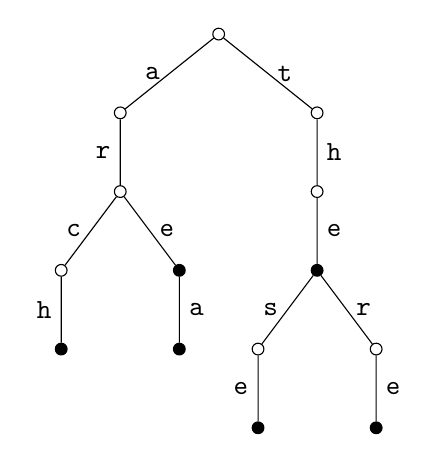
\begin{tikzpicture}[
            level distance=1cm,
            level 1/.style={sibling distance=2.5cm},
            level 2/.style={sibling distance=2cm},
            level 3/.style={sibling distance=1.5cm},
        ]
            \node[circle, draw, inner sep=1.5pt] {}
            child {
                node[circle, draw, inner sep=1.5pt] {}
                child {
                    node[circle, draw, inner sep=1.5pt] {}
                    child {
                        node[circle, draw, inner sep=1.5pt] {}
                        child {
                            node[circle, draw, fill, inner sep=1.5pt] {}
                            edge from parent node[left] {\texttt{h}}
                        }
                        edge from parent node[left] {\texttt{c}}
                    }
                    child {
                        node[circle, draw, fill, inner sep=1.5pt] {}
                        child {
                            node[circle, draw, fill, inner sep=1.5pt] {}
                            edge from parent node[right] {\texttt{a}}
                        }
                        edge from parent node[right] {\texttt{e}}
                    }
                    edge from parent node[left] {\texttt{r}}
                }
                edge from parent node[left] {\texttt{a}}
            }
            child {
                node[circle, draw, inner sep=1.5pt] {}
                child {
                    node[circle, draw, inner sep=1.5pt] {}
                    child {
                        node[circle, draw, fill, inner sep=1.5pt] {}
                        child {
                            node[circle, draw, inner sep=1.5pt] {}
                            child {
                                node[circle, draw, fill, inner sep=1.5pt] {}
                                edge from parent node[left] {\texttt{e}}
                            }
                            edge from parent node[left] {\texttt{s}}
                        }
                        child {
                            node[circle, draw, inner sep=1.5pt] {}
                            child {
                                node[circle, draw, fill, inner sep=1.5pt] {}
                                edge from parent node[right] {\texttt{e}}
                            }
                            edge from parent node[right] {\texttt{r}}
                        }
                        edge from parent node[right] {\texttt{e}}
                    }
                    edge from parent node[right] {\texttt{h}}
                }
                edge from parent node[right] {\texttt{t}}
            };
        \end{tikzpicture}
    \end{figure}
    \noindent We mark by black any node that corresponds to a string.

    A suffix trie is a trie that stores all the suffixes of a given string. For example, the suffix trie of \texttt{queue} is given below.
    \begin{figure}[H]
        \centering
        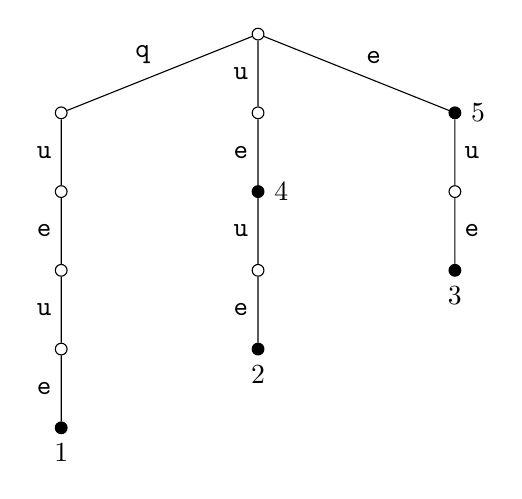
\begin{tikzpicture}[
            level distance=1cm,
            level 1/.style={sibling distance=2.5cm},
            level 2/.style={sibling distance=2cm},
            level 3/.style={sibling distance=1.5cm},
        ]
            \node[circle, draw, inner sep=1.5pt] {}
            child {
                node[circle, draw, inner sep=1.5pt] {}
                child {
                    node[circle, draw, inner sep=1.5pt] {}
                    child {
                        node[circle, draw, inner sep=1.5pt] {}
                        child {
                            node[circle, draw, inner sep=1.5pt] {}
                            child {
                                node[circle, fill, draw, inner sep=1.5pt, label={-90:1}] {}
                                edge from parent node[left] {\texttt{e}}
                            }
                            edge from parent node[left] {\texttt{u}}
                        }
                        edge from parent node[left] {\texttt{e}}
                    }
                    edge from parent node[left] {\texttt{u}}
                }
                edge from parent node[above left] {\texttt{q}}
            }
            child {
                node[circle, draw, inner sep=1.5pt] {}
                child {
                    node[circle, fill, draw, inner sep=1.5pt, label={0:4}] {}
                    child {
                        node[circle, draw, inner sep=1.5pt] {}
                        child {
                            node[circle, fill, draw, inner sep=1.5pt, label={-90:2}] {}
                            edge from parent node[left] {\texttt{e}}
                        }
                        edge from parent node[left] {\texttt{u}}
                    }
                    edge from parent node[left] {\texttt{e}}
                }
                edge from parent node[left] {\texttt{u}}
            }
            child {
                node[circle, fill, draw, inner sep=1.5pt, label={0:5}] {}
                child {
                    node[circle, draw, inner sep=1.5pt] {}
                    child {
                        node[circle, fill, draw, inner sep=1.5pt, label={-90:3}] {}
                        edge from parent node[right] {\texttt{e}}
                    }
                    edge from parent node[right] {\texttt{u}}
                }
                edge from parent node[above right] {\texttt{e}}
            };
        \end{tikzpicture}
    \end{figure}
    \noindent For a suffix trie, we also want each suffix to end at a leaf node. This is not the case in the trie above- the suffixes \texttt{ue} and \texttt{e} end at branch nodes. This is because there is a suffix (\texttt{ue}) that is a prefix of another one (\texttt{ueue}). To fix this issue, we add a unique termination symbol \texttt{\$} that is not present in the alphabet. This ensures that no suffix is a prefix of another suffix. In this case, the suffix trie for \texttt{queue} is the following:
    \begin{figure}[H]
        \centering
        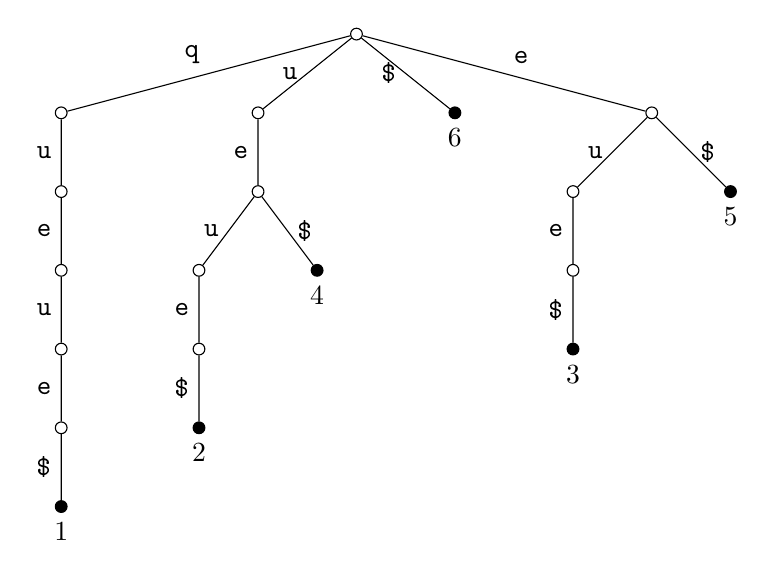
\begin{tikzpicture}[
            level distance=1cm,
            level 1/.style={sibling distance=2.5cm},
            level 2/.style={sibling distance=2cm},
            level 3/.style={sibling distance=1.5cm},
        ]
            \node[circle, draw, inner sep=1.5pt] {}
            child {
                node[circle, draw, inner sep=1.5pt] {}
                child {
                    node[circle, draw, inner sep=1.5pt] {}
                    child {
                        node[circle, draw, inner sep=1.5pt] {}
                        child {
                            node[circle, draw, inner sep=1.5pt] {}
                            child {
                                node[circle, draw, inner sep=1.5pt] {}
                                child {
                                    node[circle, fill, draw, inner sep=1.5pt, label={-90:1}] {}
                                    edge from parent node[left] {\texttt{\$}}
                                }
                                edge from parent node[left] {\texttt{e}}
                            }
                            edge from parent node[left] {\texttt{u}}
                        }
                        edge from parent node[left] {\texttt{e}}
                    }
                    edge from parent node[left] {\texttt{u}}
                }
                edge from parent node[above left] {\texttt{q}}
            }
            child {
                node[circle, draw, inner sep=1.5pt] {}
                child {
                    node[circle, draw, inner sep=1.5pt] {}
                    child {
                        node[circle, draw, inner sep=1.5pt] {}
                        child {
                            node[circle, draw, inner sep=1.5pt] {}
                            child {
                                node[circle, fill, draw, inner sep=1.5pt, label={-90:2}] {}
                                edge from parent node[left] {\texttt{\$}}
                            }
                            edge from parent node[left] {\texttt{e}}
                        }
                        edge from parent node[left] {\texttt{u}}
                    }
                    child {
                        node[circle, fill, draw, inner sep=1.5pt, label={-90:4}] {}
                        edge from parent node[right] {\texttt{\$}}
                    }
                    edge from parent node[left] {\texttt{e}}
                }
                edge from parent node[left] {\texttt{u}}
            }            
            child {
                node[circle, fill, draw, inner sep=1.5pt, label={-90:6}] {}
                edge from parent node[left] {\texttt{\$}}
            }
            child {
                node[circle, draw, inner sep=1.5pt] {}
                child {
                    node[circle, draw, inner sep=1.5pt] {}
                    child {
                        node[circle, draw, inner sep=1.5pt] {}
                        child {
                            node[circle, fill, draw, inner sep=1.5pt, label={-90:3}] {}
                            edge from parent node[left] {\texttt{\$}}
                        }
                        edge from parent node[left] {\texttt{e}}
                    }
                    edge from parent node[left] {\texttt{u}}
                }
                child {
                    node[circle, fill, draw, inner sep=1.5pt, label={-90:5}] {}
                    edge from parent node[right] {\texttt{\$}}
                }
                edge from parent node[above right] {\texttt{e}}
            };
        \end{tikzpicture}
    \end{figure}

    We will now use the suffix trie above to find \texttt{ue}. We use the suffix trie to descend from the root to the branch corresponding to the character \texttt{u}.
    \begin{figure}[H]
        \centering
        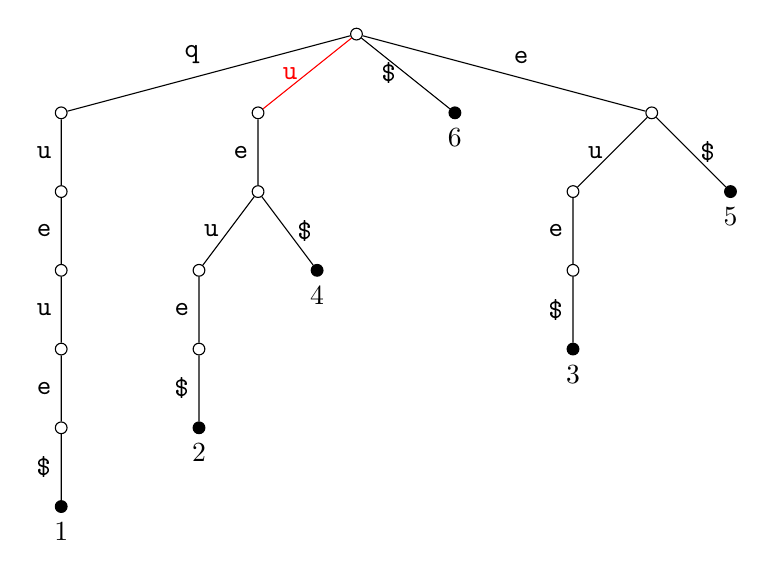
\begin{tikzpicture}[
            level distance=1cm,
            level 1/.style={sibling distance=2.5cm},
            level 2/.style={sibling distance=2cm},
            level 3/.style={sibling distance=1.5cm},
        ]
            \node[circle, draw, inner sep=1.5pt] {}
            child {
                node[circle, draw, inner sep=1.5pt] {}
                child {
                    node[circle, draw, inner sep=1.5pt] {}
                    child {
                        node[circle, draw, inner sep=1.5pt] {}
                        child {
                            node[circle, draw, inner sep=1.5pt] {}
                            child {
                                node[circle, draw, inner sep=1.5pt] {}
                                child {
                                    node[circle, fill, draw, inner sep=1.5pt, label={-90:1}] {}
                                    edge from parent node[left] {\texttt{\$}}
                                }
                                edge from parent node[left] {\texttt{e}}
                            }
                            edge from parent node[left] {\texttt{u}}
                        }
                        edge from parent node[left] {\texttt{e}}
                    }
                    edge from parent node[left] {\texttt{u}}
                }
                edge from parent node[above left] {\texttt{q}}
            }
            child {
                node[circle, draw, inner sep=1.5pt] {}
                child {
                    node[circle, draw, black, inner sep=1.5pt] {}
                    child {
                        node[circle, draw, inner sep=1.5pt] {}
                        child {
                            node[circle, draw, inner sep=1.5pt] {}
                            child {
                                node[circle, fill, draw, inner sep=1.5pt, label={-90:2}] {}
                                edge from parent node[left] {\texttt{\$}}
                            }
                            edge from parent node[left] {\texttt{e}}
                        }
                        edge from parent[black] node[left] {\texttt{u}}
                    }
                    child {
                        node[circle, fill, draw, inner sep=1.5pt, label={-90:4}] {}
                        edge from parent node[right] {\texttt{\$}}
                    }
                    edge from parent[black] node[left] {\texttt{e}}
                }
                edge from parent[red] node[left] {\texttt{u}}
            }            
            child {
                node[circle, fill, draw, inner sep=1.5pt, label={-90:6}] {}
                edge from parent node[left] {\texttt{\$}}
            }
            child {
                node[circle, draw, inner sep=1.5pt] {}
                child {
                    node[circle, draw, inner sep=1.5pt] {}
                    child {
                        node[circle, draw, inner sep=1.5pt] {}
                        child {
                            node[circle, fill, draw, inner sep=1.5pt, label={-90:3}] {}
                            edge from parent node[left] {\texttt{\$}}
                        }
                        edge from parent node[left] {\texttt{e}}
                    }
                    edge from parent node[left] {\texttt{u}}
                }
                child {
                    node[circle, fill, draw, inner sep=1.5pt, label={-90:5}] {}
                    edge from parent node[right] {\texttt{\$}}
                }
                edge from parent node[above right] {\texttt{e}}
            };
        \end{tikzpicture}
    \end{figure}
    \noindent We then descend from this branch to the one corresponding to the character \texttt{e}.
    \begin{figure}[H]
        \centering
        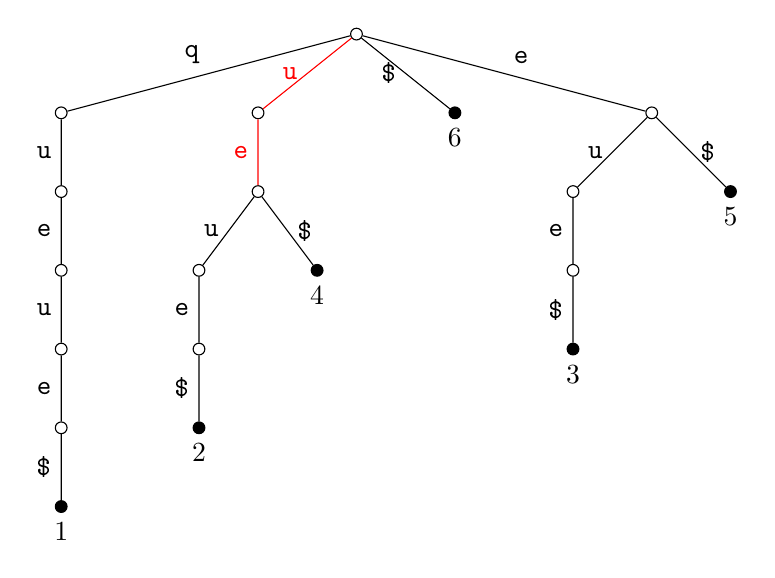
\begin{tikzpicture}[
            level distance=1cm,
            level 1/.style={sibling distance=2.5cm},
            level 2/.style={sibling distance=2cm},
            level 3/.style={sibling distance=1.5cm},
        ]
            \node[circle, draw, inner sep=1.5pt] {}
            child {
                node[circle, draw, inner sep=1.5pt] {}
                child {
                    node[circle, draw, inner sep=1.5pt] {}
                    child {
                        node[circle, draw, inner sep=1.5pt] {}
                        child {
                            node[circle, draw, inner sep=1.5pt] {}
                            child {
                                node[circle, draw, inner sep=1.5pt] {}
                                child {
                                    node[circle, fill, draw, inner sep=1.5pt, label={-90:1}] {}
                                    edge from parent node[left] {\texttt{\$}}
                                }
                                edge from parent node[left] {\texttt{e}}
                            }
                            edge from parent node[left] {\texttt{u}}
                        }
                        edge from parent node[left] {\texttt{e}}
                    }
                    edge from parent node[left] {\texttt{u}}
                }
                edge from parent node[above left] {\texttt{q}}
            }
            child {
                node[circle, draw, inner sep=1.5pt] {}
                child {
                    node[circle, draw, black, inner sep=1.5pt] {}
                    child {
                        node[circle, draw, black, inner sep=1.5pt] {}
                        child {
                            node[circle, draw, black, inner sep=1.5pt] {}
                            child {
                                node[circle, fill, draw, inner sep=1.5pt, label={-90:2}] {}
                                edge from parent node[left] {\texttt{\$}}
                            }
                            edge from parent node[left] {\texttt{e}}
                        }
                        edge from parent[black] node[left] {\texttt{u}}
                    }
                    child {
                        node[circle, fill, draw, black, inner sep=1.5pt, label={-90:4}] {}
                        edge from parent[black]  node[right] {\texttt{\$}}
                    }
                    edge from parent[red] node[left] {\texttt{e}}
                }
                edge from parent[red] node[left] {\texttt{u}}
            }            
            child {
                node[circle, fill, draw, inner sep=1.5pt, label={-90:6}] {}
                edge from parent node[left] {\texttt{\$}}
            }
            child {
                node[circle, draw, inner sep=1.5pt] {}
                child {
                    node[circle, draw, inner sep=1.5pt] {}
                    child {
                        node[circle, draw, inner sep=1.5pt] {}
                        child {
                            node[circle, fill, draw, inner sep=1.5pt, label={-90:3}] {}
                            edge from parent node[left] {\texttt{\$}}
                        }
                        edge from parent node[left] {\texttt{e}}
                    }
                    edge from parent node[left] {\texttt{u}}
                }
                child {
                    node[circle, fill, draw, inner sep=1.5pt, label={-90:5}] {}
                    edge from parent node[right] {\texttt{\$}}
                }
                edge from parent node[above right] {\texttt{e}}
            };
        \end{tikzpicture}
    \end{figure}
    \noindent We have now completely matched the substring. This means that the substring occurs at indices 2 and 4. Using the suffix trie, we were able to find all the occurrences in linear time with respect to the substring (assuming that the alphabet has constant size). If we had tried to match \texttt{ux} instead, we would not have been able to find a branch for the second letter. That implies that there is no match in the string. 

    We can use the suffix trie to also find the longest repeated substring. This corresponds to finding the branch node with the greatest string depth. A branch node is a prefix of at least 2 suffixes, and so represents a repeated substring. For the string \texttt{queue}, the repeated substrings, as seen in the trie, are \texttt{e} and \texttt{ue}. Hence, the longest repeated substring is \texttt{ue}, with length 2, with starting indices 2 and 4.

    To build a suffix trie, we repeated insert all the suffixes to the trie. To insert the suffix $i$, it takes $O(n-i)$ time. So, overall, it takes $O(n^2)$ time and space. This is not tractable for long texts. To improve this, we make use of suffix trees.

    \subsection{Suffix Trees}
    Suffix trees are very similar to suffix tries, but we have compressed unary branch nodes. So, the suffix tree for \texttt{queue} is the following:
    \begin{figure}[H]
        \centering
        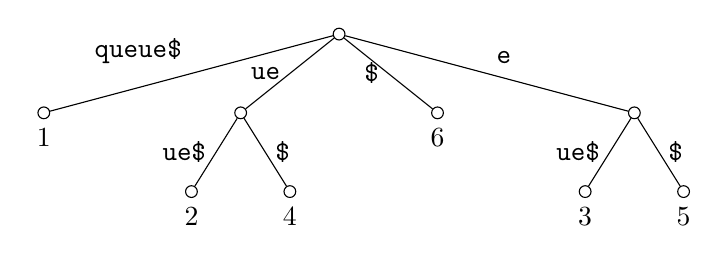
\begin{tikzpicture}[
            level distance=1cm,
            level 1/.style={sibling distance=2.5cm},
            level 2/.style={sibling distance=1.25cm},
            level 3/.style={sibling distance=0.5cm},
        ]
            \node[circle, draw, inner sep=1.5pt] {}
            child {
                node[circle, draw, inner sep=1.5pt, label={-90:1}] {}
                edge from parent node[above left] {\texttt{queue\$}}
            }
            child {
                node[circle, draw, inner sep=1.5pt] {}
                child {
                    node[circle, draw, inner sep=1.5pt, label={-90:2}] {}
                    edge from parent node[left] {\texttt{ue\$}}
                }
                child {
                    node[circle, draw, inner sep=1.5pt, label={-90:4}] {}
                    edge from parent node[right] {\texttt{\$}}
                }
                edge from parent node[left] {\texttt{ue}}
            }            
            child {
                node[circle, draw, inner sep=1.5pt, label={-90:6}] {}
                edge from parent node[left] {\texttt{\$}}
            }
            child {
                node[circle, draw, inner sep=1.5pt] {}
                child {
                    node[circle, draw, inner sep=1.5pt, label={-90:3}] {}
                    edge from parent node[left] {\texttt{ue\$}}
                }
                child {
                    node[circle, draw, inner sep=1.5pt, label={-90:5}] {}
                    edge from parent node[right] {\texttt{\$}}
                }
                edge from parent node[above right] {\texttt{e}}
            };
        \end{tikzpicture}
    \end{figure}    
    \noindent This is a much more efficient representation since we do not need to store a node for each letter. In this case, the number of nodes is $O(n)$, whereas for the suffix trie, it was $O(n^2)$.

    Now, we define the suffix tree for some string $S$. We first append $\$$ to the string and construct all the suffixes that satisfy the following properties:
    \begin{itemize}
        \item each edge has a string label;
        \item all branch nodes have at most 2 children;
        \item no two children of a branch node have two edges that started with the same character;
        \item there is a bijection between the leaf nodes and the suffixes, i.e. we can descend from the root to a leaf to recover the suffix. The entire label (from root to a node) is called its \emph{path label}.
    \end{itemize}

    In a suffix tree, there are $n+1$ suffixes, so $n+1$ leaf nodes. Also, the number of branch nodes is at most $n$. To see this, assume that we have $x$ edges, $n$ leaf nodes and $b$ branches. Then, $x = b + n - 1$- we have an edge going to each branch node and leaf node, except for the root. Moreover, since every branch node has at least 2 children, $x \geq 2b$. Hence, $b \leq n - 1$. Hence, there are $O(n)$ nodes in total. This is an improvement from suffix tries, which have $O(n^2)$ nodes.
    
    However, the suffix tree still has $O(n^2)$ space complexity- we need linear space to store the entire suffix. To mitigate this, we just store the index of the start and the end of the substring in the text. So, the suffix tree for \texttt{queue} is the following:    
    \begin{figure}[H]
        \centering
        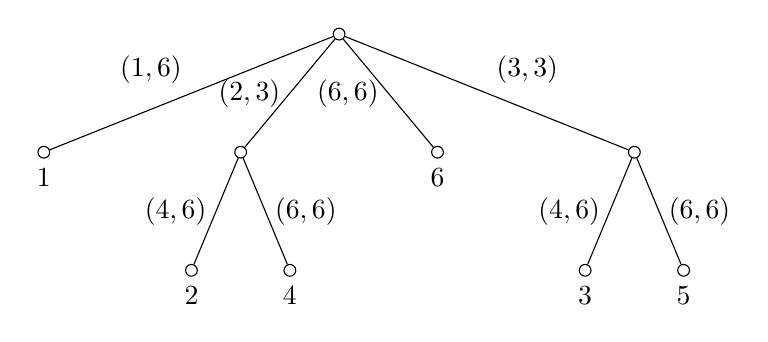
\begin{tikzpicture}[
            level distance=1.5cm,
            level 1/.style={sibling distance=2.5cm},
            level 2/.style={sibling distance=1.25cm},
            level 3/.style={sibling distance=0.5cm},
        ]
            \node[circle, draw, inner sep=1.5pt] {}
            child {
                node[circle, draw, inner sep=1.5pt, label={-90:1}] {}
                edge from parent node[above left] {$(1, 6)$}
            }
            child {
                node[circle, draw, inner sep=1.5pt] {}
                child {
                    node[circle, draw, inner sep=1.5pt, label={-90:2}] {}
                    edge from parent node[left] {$(4, 6)$}
                }
                child {
                    node[circle, draw, inner sep=1.5pt, label={-90:4}] {}
                    edge from parent node[right] {$(6, 6)$}
                }
                edge from parent node[left] {$(2, 3)$}
            }            
            child {
                node[circle, draw, inner sep=1.5pt, label={-90:6}] {}
                edge from parent node[left] {$(6, 6)$}
            }
            child {
                node[circle, draw, inner sep=1.5pt] {}
                child {
                    node[circle, draw, inner sep=1.5pt, label={-90:3}] {}
                    edge from parent node[left] {$(4, 6)$}
                }
                child {
                    node[circle, draw, inner sep=1.5pt, label={-90:5}] {}
                    edge from parent node[right] {$(6, 6)$}
                }
                edge from parent node[above right] {$(3, 3)$}
            };
        \end{tikzpicture}
    \end{figure}
    \noindent Each label now takes $O(1)$ space, so the total complexity is $O(n)$ space. We call this representation the \emph{suffix tree with short edge labels}, and the one above as the \emph{suffix tree with full edge labels}.

    One way to construct the suffix tree with short edge labels is to create the suffix trie, use it to construct the suffix tree with full edge labels by collapsing unary branches, and then replace the full edge labels with short edge labels. This is not the most efficient approach since we do need $O(n^2)$ space during the algorithm.

    A more efficient approach would involve directly constructing the suffix tree with short edge labels. We illustrate this with an example, by constructing the suffix tree with full edge labels for \texttt{queue}. We will use full edge labels for illustration purposes; the algorithm would instead make use of the short edge labels. We start by inserting the suffix \texttt{queue\$}.
    \begin{figure}[H]
        \centering
        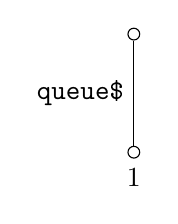
\begin{tikzpicture}[
            level distance=1.5cm,
            level 1/.style={sibling distance=2.5cm},
            level 2/.style={sibling distance=1.25cm},
            level 3/.style={sibling distance=0.5cm},
        ]
            \node[circle, draw, inner sep=1.5pt] {}
            child {
                node[circle, draw, inner sep=1.5pt, label={-90:1}] {}
                edge from parent node[left] {\texttt{queue\$}}
            };
        \end{tikzpicture}
    \end{figure}
    \noindent We insert the suffix by branching from the root. We can do the same thing when inserting the next two suffixes- \texttt{ueue\$} and \texttt{eue\$}.
    \begin{figure}[H]
        \centering
        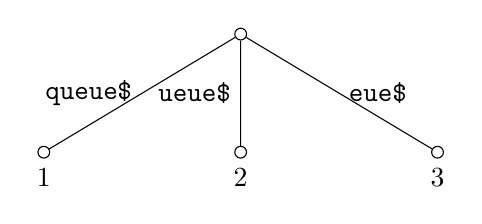
\begin{tikzpicture}[
            level distance=1.5cm,
            level 1/.style={sibling distance=2.5cm},
            level 2/.style={sibling distance=1.25cm},
            level 3/.style={sibling distance=0.5cm},
        ]
            \node[circle, draw, inner sep=1.5pt] {}
            child {
                node[circle, draw, inner sep=1.5pt, label={-90:1}] {}
                edge from parent node[left] {\texttt{queue\$}}
            }
            child {
                node[circle, draw, inner sep=1.5pt, label={-90:2}] {}
                edge from parent node[left] {\texttt{ueue\$}}
            }
            child {
                node[circle, draw, inner sep=1.5pt, label={-90:3}] {}
                edge from parent node[right] {\texttt{eue\$}}
            };
        \end{tikzpicture}
    \end{figure}
    \noindent At this point, the next suffix is \texttt{ue\$}. We already have a node starting with \texttt{ue}, but this is not a complete match (i.e. the branch has a longer label). So, we perform an \emph{edge-split} first to ensure we can branch at the right position.
    \begin{figure}[H]
        \centering
        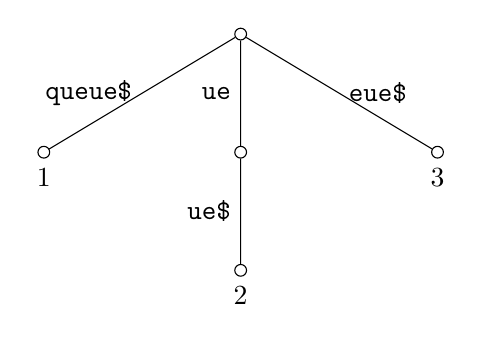
\begin{tikzpicture}[
            level distance=1.5cm,
            level 1/.style={sibling distance=2.5cm},
            level 2/.style={sibling distance=1.25cm},
            level 3/.style={sibling distance=0.5cm},
        ]
            \node[circle, draw, inner sep=1.5pt] {}
            child {
                node[circle, draw, inner sep=1.5pt, label={-90:1}] {}
                edge from parent node[left] {\texttt{queue\$}}
            }
            child {
                node[circle, draw, inner sep=1.5pt] {}
                child {
                    node[circle, draw, inner sep=1.5pt, label={-90:2}] {}
                    edge from parent node[left] {\texttt{ue\$}}
                }
                edge from parent node[left] {\texttt{ue}}
            }
            child {
                node[circle, draw, inner sep=1.5pt, label={-90:3}] {}
                edge from parent node[right] {\texttt{eue\$}}
            };
        \end{tikzpicture}
    \end{figure}
    \noindent We can now insert \texttt{ue\$} as a child of the branch \texttt{ue}.    
    \begin{figure}[H]
        \centering
        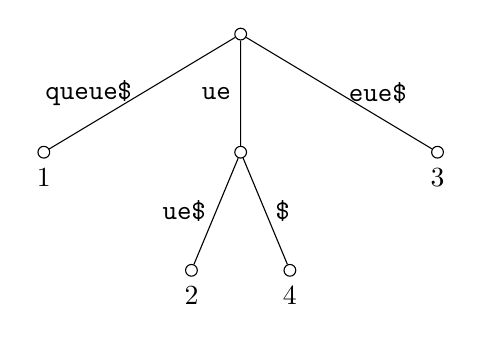
\begin{tikzpicture}[
            level distance=1.5cm,
            level 1/.style={sibling distance=2.5cm},
            level 2/.style={sibling distance=1.25cm},
            level 3/.style={sibling distance=0.5cm},
        ]
            \node[circle, draw, inner sep=1.5pt] {}
            child {
                node[circle, draw, inner sep=1.5pt, label={-90:1}] {}
                edge from parent node[left] {\texttt{queue\$}}
            }
            child {
                node[circle, draw, inner sep=1.5pt] {}
                child {
                    node[circle, draw, inner sep=1.5pt, label={-90:2}] {}
                    edge from parent node[left] {\texttt{ue\$}}
                }                
                child {
                    node[circle, draw, inner sep=1.5pt, label={-90:4}] {}
                    edge from parent node[right] {\texttt{\$}}
                }
                edge from parent node[left] {\texttt{ue}}
            }
            child {
                node[circle, draw, inner sep=1.5pt, label={-90:3}] {}
                edge from parent node[right] {\texttt{eue\$}}
            };
        \end{tikzpicture}
    \end{figure}
    \noindent We have to do the same thing when inserting \texttt{e\$}- we edge-split \texttt{eue\$}.    
    \begin{figure}[H]
        \centering
        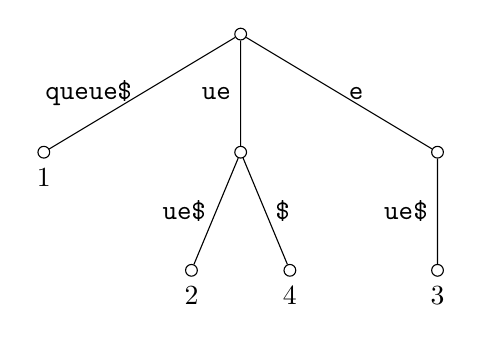
\begin{tikzpicture}[
            level distance=1.5cm,
            level 1/.style={sibling distance=2.5cm},
            level 2/.style={sibling distance=1.25cm},
            level 3/.style={sibling distance=0.5cm},
        ]
            \node[circle, draw, inner sep=1.5pt] {}
            child {
                node[circle, draw, inner sep=1.5pt, label={-90:1}] {}
                edge from parent node[left] {\texttt{queue\$}}
            }
            child {
                node[circle, draw, inner sep=1.5pt] {}
                child {
                    node[circle, draw, inner sep=1.5pt, label={-90:2}] {}
                    edge from parent node[left] {\texttt{ue\$}}
                }                
                child {
                    node[circle, draw, inner sep=1.5pt, label={-90:4}] {}
                    edge from parent node[right] {\texttt{\$}}
                }
                edge from parent node[left] {\texttt{ue}}
            }
            child {
                node[circle, draw, inner sep=1.5pt] {}
                child {
                    node[circle, draw, inner sep=1.5pt, label={-90:3}] {}
                    edge from parent node[left] {\texttt{ue\$}}
                }
                edge from parent node[right] {\texttt{e}}
            };
        \end{tikzpicture}
    \end{figure}
    \noindent We can now insert \texttt{e\$} to the tree.
    \begin{figure}[H]
        \centering
        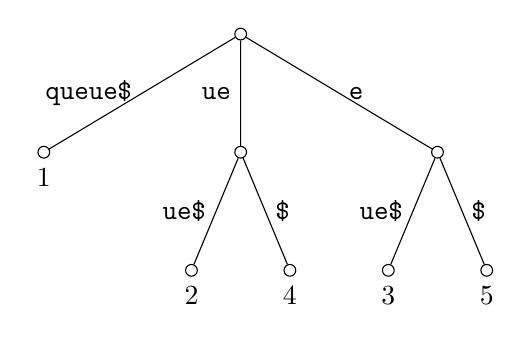
\begin{tikzpicture}[
            level distance=1.5cm,
            level 1/.style={sibling distance=2.5cm},
            level 2/.style={sibling distance=1.25cm},
            level 3/.style={sibling distance=0.5cm},
        ]
            \node[circle, draw, inner sep=1.5pt] {}
            child {
                node[circle, draw, inner sep=1.5pt, label={-90:1}] {}
                edge from parent node[left] {\texttt{queue\$}}
            }
            child {
                node[circle, draw, inner sep=1.5pt] {}
                child {
                    node[circle, draw, inner sep=1.5pt, label={-90:2}] {}
                    edge from parent node[left] {\texttt{ue\$}}
                }                
                child {
                    node[circle, draw, inner sep=1.5pt, label={-90:4}] {}
                    edge from parent node[right] {\texttt{\$}}
                }
                edge from parent node[left] {\texttt{ue}}
            }
            child {
                node[circle, draw, inner sep=1.5pt] {}
                child {
                    node[circle, draw, inner sep=1.5pt, label={-90:3}] {}
                    edge from parent node[left] {\texttt{ue\$}}
                }
                child {
                    node[circle, draw, inner sep=1.5pt, label={-90:5}] {}
                    edge from parent node[right] {\texttt{\$}}
                }
                edge from parent node[right] {\texttt{e}}
            };
        \end{tikzpicture}
    \end{figure}
    \noindent Next, we insert \texttt{\$}.
    \begin{figure}[H]
        \centering
        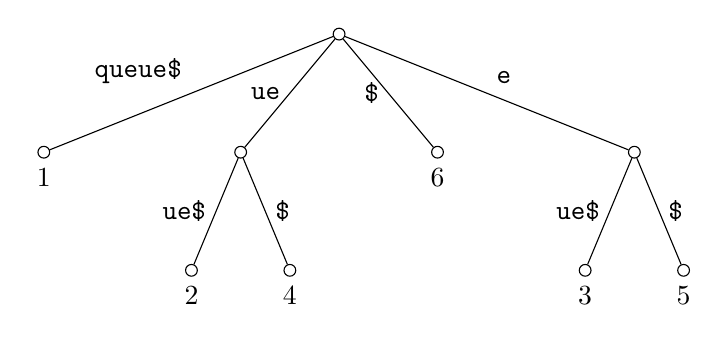
\begin{tikzpicture}[
            level distance=1.5cm,
            level 1/.style={sibling distance=2.5cm},
            level 2/.style={sibling distance=1.25cm},
            level 3/.style={sibling distance=0.5cm},
        ]
            \node[circle, draw, inner sep=1.5pt] {}
            child {
                node[circle, draw, inner sep=1.5pt, label={-90:1}] {}
                edge from parent node[above left] {\texttt{queue\$}}
            }
            child {
                node[circle, draw, inner sep=1.5pt] {}
                child {
                    node[circle, draw, inner sep=1.5pt, label={-90:2}] {}
                    edge from parent node[left] {\texttt{ue\$}}
                }
                child {
                    node[circle, draw, inner sep=1.5pt, label={-90:4}] {}
                    edge from parent node[right] {\texttt{\$}}
                }
                edge from parent node[left] {\texttt{ue}}
            }            
            child {
                node[circle, draw, inner sep=1.5pt, label={-90:6}] {}
                edge from parent node[left] {\texttt{\$}}
            }
            child {
                node[circle, draw, inner sep=1.5pt] {}
                child {
                    node[circle, draw, inner sep=1.5pt, label={-90:3}] {}
                    edge from parent node[left] {\texttt{ue\$}}
                }
                child {
                    node[circle, draw, inner sep=1.5pt, label={-90:5}] {}
                    edge from parent node[right] {\texttt{\$}}
                }
                edge from parent node[above right] {\texttt{e}}
            };
        \end{tikzpicture}
    \end{figure}
    \noindent The suffix tree is now complete.

    This algorithm takes $O(n)$ space complexity, but has worst-case complexity $O(n^2)$, e.g. if we have to edge-split every time. The average case is $O(n \log n)$. There are more efficient algorithms that require $O(n)$ time complexity.

    We will now use the suffix tree for different string algorithms. If we have a string $S$ and a substring $T$ to search in the string, we construct a tree on $S$, and then match each letter in $T$ with the corresponding node. If we cannot match $T$ completely, then the string is not present. If it is present, we can return the index of the match by using the branch node we are at. This algorithm is very similar to the one for suffix tries we saw above. The time taken for this algorithm is linear with respect to the substring. We can also find all occurrences using this approach.

    Now, we try to find the longest repeated substring in a text $S$. We can construct the suffix tree for $S$ in $O(n)$ time. We then traverse the tree to find the branch node with the greatest string depth. A branch node corresponds to a common substring, and the string depth keeps track of the length of the common substring. We can traverse in $O(n)$ time, so the entire algorithm is $O(n)$.

    Next, we can find a longest common substring of texts $S$ and $T$. To do so, we construct the suffix tree for $S\#T\$$, where $\#$ and $\$$ are symbols not in $\Sigma$. This is called the \emph{generalised suffix tree}. We then traverse the tree in a similar way as the longest repeated substring, but we are looking for a common branch node with the greatest string depth. A common branch is one that has leaf nodes corresponding to suffix starting in both $S$ and $T$.

    Now, we will look at a method to identify common branch nodes. For each branch node $v$, we keep track of two values- whether it has a leaf node with suffix value corresponding to a string in $S$ ($b_1(v)$), and whether it has a leaf node with suffix value corresponding to a string in $T$ ($b_2(v)$). Then, $v$ is a branch node if and only if $b_1(v) \land b_2(v)$. We can compute the $b_i(v)$ values as follows:
    \begin{itemize}
        \item if $v$ is a leaf node, then we can check the value of the suffix to compute $b_i(v)$- $b_1(v)$ is \texttt{true} if $1 \leq j \leq m$ and $b_2(v)$ is \texttt{true} if $m+2 \leq j \leq m+n+1$, where $m$ and $n$ are the lengths of $S$ and $T$ respectively;
        \item instead, if $v$ is a branch node, then $b_i(v) = b_i(w_1) \land b_i(w_2) \land \dots \land b_i(w_n)$, where $w_1, w_2, \dots, w_n$ are the descendant leaf nodes of $v$. 
    \end{itemize}

    So, the algorithm for longest common substring is the following:
    \begin{itemize}
        \item build the generalised suffix tree;
        \item calculate the values $b_i(v)$ for every node $v$;
        \item find the common branch node with maximum string depth.
    \end{itemize}
    The last 2 steps can be combined. Each step takes $O(m+n)$ time, so the algorithm overall takes $O(m+n)$ time.

    We will now illustrate that the character $\#$ is required in order to correctly output the result. So, assume that the two strings are \texttt{a} and \texttt{bab}. Then, the suffix tree for $ST\$$ is the following:
    \begin{figure}[H]
        \centering
        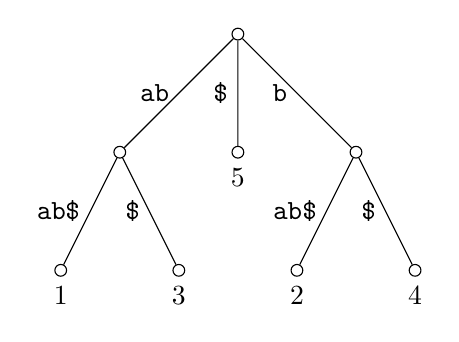
\begin{tikzpicture}
            \node[circle, draw, inner sep=1.5pt] {}
            child {
                node[circle, draw, inner sep=1.5pt] {}
                child {
                    node[circle, draw, inner sep=1.5pt, label={-90:1}] {}
                    edge from parent node[left] {\texttt{ab\$}}
                }
                child {
                    node[circle, draw, inner sep=1.5pt, label={-90:3}] {}
                    edge from parent node[left] {\texttt{\$}}
                }
                edge from parent node[left] {\texttt{ab}}
            }
            child {
                node[circle, draw, inner sep=1.5pt, label={-90:5}] {}
                edge from parent node[left] {\texttt{\$}}
            }
            child {
                node[circle, draw, inner sep=1.5pt] {}
                child {
                    node[circle, draw, inner sep=1.5pt, label={-90:2}] {}
                    edge from parent node[left] {\texttt{ab\$}}
                }
                child {
                    node[circle, draw, inner sep=1.5pt, label={-90:4}] {}
                    edge from parent node[left] {\texttt{\$}}
                }
                edge from parent node[left] {\texttt{b}}
            };
        \end{tikzpicture}
    \end{figure}
    \noindent Here, the common branch node with the greatest depth is \texttt{ab}. However, it is not a common substring of \texttt{a} and \texttt{bab}.
    \newpage

    \section{Matching Regular Expressions}
    In this section, we will look at searching a regular expressions in some text. There are many algorithms to search a string in some text, including brute-force, KMP, BM and suffix trees. We will generalise the brute-force algorithm to match regular expressions.

    A \emph{regular expression} represents a set of strings on some alphabet $\Sigma$, called a \emph{language}. For example, if the regular expression is \texttt{a|b}, then the language is: $\{\texttt{a}, \texttt{b}\}$. We say that a string \emph{matches} a regular expression if it is an element of the language.

    We will now define regular expressions over some alphabet $\Sigma$.
    \begin{itemize}
        \item the empty string $\epsilon$ is a regular expression, with language $\{\epsilon\}$;
        \item for a character $\sigma \in \Sigma$, $\sigma$ is a regular expression, with language $\{\sigma\}$;
        \item for regular expressions \texttt{R} and \texttt{S} with languages $L_{\texttt{R}}$ and $L_{\texttt{S}}$, their concatenation \texttt{RS} is a regular expression with language
        \[L_{\texttt{RS}} = \{XY \mid X \in L_{\texttt{R}}, Y \in L_{\texttt{S}}\}.\]
        \item for regular expressions \texttt{R} and \texttt{S} with languages $L_{\texttt{R}}$ and $L_{\texttt{S}}$, their choice \texttt{R|S} is a regular expression, with language $L_{\texttt{R|S}} = L_{\texttt{R}} \cup L_{\texttt{S}}$.
        \item for a regular expression \texttt{R} with language $L_{\texttt{R}}$, its closure $\texttt{R}^*$ is a regular expression, with language 
        \[L_{\texttt{R}^*} = \{\epsilon\} \cup \{XY \mid X \in L_{\texttt{R}}, Y \in L_{\texttt{R}^*}\}.\]
        \item for a regular expression \texttt{R} with language $L_{\texttt{R}}$, its bracketed form \texttt{(R)} is a regular expression with language $L_{\texttt{(R)}} = L_{\texttt{R}}$.
    \end{itemize}

    When we unpack a regular expression, the following is the order of precedence:
    \begin{itemize}
        \item the bracket has the highest precedence (and can be used to override any of the precedence rule below);
        \item the closure operation;
        \item the concatenation operation; and
        \item the choice operation.
    \end{itemize}
    Hence, the regular expression $\texttt{ab}^*\texttt{d}$ has the language
    \[\{\texttt{ad}, \texttt{abd}, \texttt{abbd}, \dots\},\]
    while $(\texttt{ab})^* \texttt{d}$ has the language
    \[\{\texttt{d}, \texttt{abd}, \texttt{ababd}, \dots\}.\]
    There are further regular expressions such as complement \texttt{-x} which refers to all characters in $\Sigma$ except \texttt{x}, and \texttt{?} which corresponds to any character in $\Sigma$.

    We will now look at the problem- given a text \texttt{T} and a regular expression \texttt{R}, check whether \texttt{T} matches \texttt{R}. The algorithm we will look at considers each position in text, and checks whether we have had a match with a substring ending at that position. To do so, we need to keep track of all prefixes of \texttt{R} that are matched at any given position. We will use an non-deterministic finite automaton (NDFA) to do so.

    An NDFA is a directed graph with vertices, called states. There are always two states- a starting state and a halting state. The edges are called transitions, and have an label- a character in the alphabet $\Sigma$, including the empty character $\epsilon$. We say that an NDFA \emph{accepts} a string if there exists a path from the starting state to the halting state that matches all the characters in the string using the edge labels.

    Every regular expression can be represented by an NDFA, and vice versa (though neither representation is unique). For instance, an NDFA for the regular expression $\texttt{a}^*|\texttt{b}^*$ is:
    \begin{figure}[H]
        \centering
        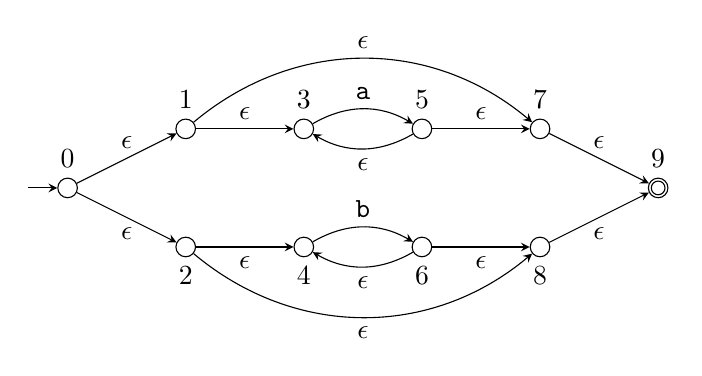
\begin{tikzpicture}
            \node[circle, draw, inner sep=2.5pt, label={90:0}] (q0) at (0, 0) {};
            \node[circle, draw, inner sep=2.5pt, label={90:1}] (q1) at (1.5, 0.75) {};
            \node[circle, draw, inner sep=2.5pt, label={-90:2}] (q2) at (1.5, -0.75) {};
            \node[circle, draw, inner sep=2.5pt, label={90:3}] (q3) at (3, 0.75) {};
            \node[circle, draw, inner sep=2.5pt, label={-90:4}] (q4) at (3, -0.75) {};
            \node[circle, draw, inner sep=2.5pt, label={90:5}] (q5) at (4.5, 0.75) {};
            \node[circle, draw, inner sep=2.5pt, label={-90:6}] (q6) at (4.5, -0.75) {};
            \node[circle, draw, inner sep=2.5pt, label={90:7}] (q7) at (6, 0.75) {};
            \node[circle, draw, inner sep=2.5pt, label={-90:8}] (q8) at (6, -0.75) {};
            \node[circle, draw, inner sep=2.5pt, label={90:9}] (q9) at (7.5, 0) {};
            \node[circle, draw, inner sep=1.75pt] at (7.5, 0) {};

            \draw[-stealth] (-0.5, 0) -- (q0);
            \draw[-stealth] (q0) edge node[above] {$\epsilon$} (q1);
            \draw[-stealth] (q0) edge node[below] {$\epsilon$} (q2);
            \draw[-stealth] (q1) edge node[above] {$\epsilon$} (q3);
            \draw[-stealth] (q2) edge node[below] {$\epsilon$} (q4);
            \draw[-stealth] (q3) edge[bend left] node[above] {\texttt{a}} (q5);
            \draw[-stealth] (q5) edge[bend left] node[below] {$\epsilon$} (q3);
            \draw[-stealth] (q4) edge[bend left] node[above] {\texttt{b}} (q6);
            \draw[-stealth] (q6) edge[bend left] node[below] {$\epsilon$} (q4);
            \draw[-stealth] (q5) edge node[above] {$\epsilon$} (q7);
            \draw[-stealth] (q6) edge node[below] {$\epsilon$} (q8);
            \draw[-stealth] (q7) edge node[above] {$\epsilon$} (q9);
            \draw[-stealth] (q8) edge node[below] {$\epsilon$} (q9);
            \draw[-stealth] (q1) edge[bend left=40] node[above] {$\epsilon$} (q7);
            \draw[-stealth] (q2) edge[bend right=40] node[below] {$\epsilon$} (q8);
        \end{tikzpicture}
    \end{figure}
    \noindent The starting state is 0, shown by an arrow coming to it. The halting state is 9, which is shown by double circle. Some of the strings it accepts are given below:
    \begin{itemize}
        \item the empty string, which can be matched by following the path: $0- 1 - 7 - 9$;
        \item the string \texttt{b}, which can be matched by following the path: $0 - 2 - 4 - 6 - 8 - 9$; and
        \item the string \texttt{aa}, which can be matched by following the path: $0 - 1 - 3 - 5 - 3 - 5 - 7 - 9$.
    \end{itemize}

    We will now systematically construct an NDFA given a regular expression. This representation will have different properties that will allow us to conclude the efficiency of the algorithm. The following is the way we construct an NDFA:
    \begin{itemize}
        \item The following is the NDFA for the empty string:
        \begin{figure}[H]
            \centering
            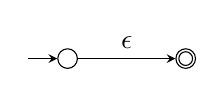
\begin{tikzpicture}
                \node[circle, draw, inner sep=2.5pt] (q0) at (0, 0) {};
                \node[circle, draw, inner sep=2.5pt] (q1) at (1.5, 0) {};
                \node[circle, draw, inner sep=1.75pt] at (1.5, 0) {};
                
                \draw[-stealth] (-0.5, 0) -- (q0);
                \draw[-stealth] (q0) edge node[above] {$\epsilon$} (q1);
            \end{tikzpicture}
        \end{figure}

        \item The following is the NDFA for a character $\sigma$:
        \begin{figure}[H]
            \centering
            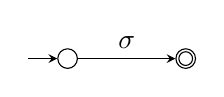
\begin{tikzpicture}
                \node[circle, draw, inner sep=2.5pt] (q0) at (0, 0) {};
                \node[circle, draw, inner sep=2.5pt] (q1) at (1.5, 0) {};
                \node[circle, draw, inner sep=1.75pt] at (1.5, 0) {};

                \draw[-stealth] (-0.5, 0) -- (q0);
                \draw[-stealth] (q0) edge node[above] {$\sigma$} (q1);
            \end{tikzpicture}
        \end{figure}

        \item Let the NDFAs for $\texttt{R}_1$ and $\texttt{R}_2$ be the following:
        \begin{figure}[H]
            \centering
            \begin{subfigure}{0.4\textwidth}
                \centering
                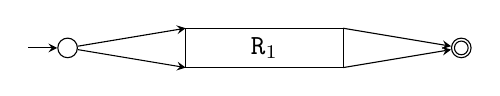
\begin{tikzpicture}
                    \node[circle, draw, inner sep=2.5pt] (q0) at (0, 0) {};
                    \draw (1.5, -0.25) rectangle (3.5, 0.25);
                    \node at (2.5, 0) {$\texttt{R}_1$};
                    \node[circle, draw, inner sep=2.5pt] (q1) at (5, 0) {};
                    \node[circle, draw, inner sep=1.75pt] at (5, 0) {};

                    \draw[-stealth] (-0.5, 0) -- (q0);
                    \draw[-stealth] (q0) -- (1.5, 0.25);
                    \draw[-stealth] (q0) -- (1.5, -0.25);
                    \draw[-stealth] (3.5, 0.25) -- (q1);
                    \draw[-stealth] (3.5, -0.25) -- (q1);
                \end{tikzpicture}
            \end{subfigure}
            \hfill
            \begin{subfigure}{0.4\textwidth}
                \centering
                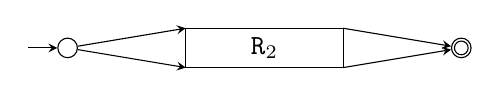
\begin{tikzpicture}
                    \node[circle, draw, inner sep=2.5pt] (q0) at (0, 0) {};
                    \draw (1.5, -0.25) rectangle (3.5, 0.25);
                    \node at (2.5, 0) {$\texttt{R}_2$};
                    \node[circle, draw, inner sep=2.5pt] (q1) at (5, 0) {};
                    \node[circle, draw, inner sep=1.75pt] at (5, 0) {};

                    \draw[-stealth] (-0.5, 0) -- (q0);
                    \draw[-stealth] (q0) -- (1.5, 0.25);
                    \draw[-stealth] (q0) -- (1.5, -0.25);
                    \draw[-stealth] (3.5, 0.25) -- (q1);
                    \draw[-stealth] (3.5, -0.25) -- (q1);
                \end{tikzpicture}
            \end{subfigure}
        \end{figure}
        Then, the NDFA for $\texttt{R}_1\texttt{R}_2$ is the following:
        \begin{figure}[H]
            \centering
            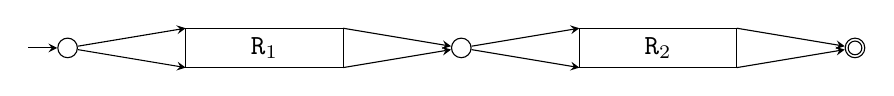
\begin{tikzpicture}
                \node[circle, draw, inner sep=2.5pt] (q0) at (0, 0) {};
                \draw (1.5, -0.25) rectangle (3.5, 0.25);
                \node at (2.5, 0) {$\texttt{R}_1$};
                \node[circle, draw, inner sep=2.5pt] (q1) at (5, 0) {};
                \draw (6.5, -0.25) rectangle (8.5, 0.25);
                \node at (7.5, 0) {$\texttt{R}_2$};
                \node[circle, draw, inner sep=2.5pt] (q2) at (10, 0) {};
                \node[circle, draw, inner sep=1.75pt] at (10, 0) {};

                \draw[-stealth] (-0.5, 0) -- (q0);
                \draw[-stealth] (q0) -- (1.5, 0.25);
                \draw[-stealth] (q0) -- (1.5, -0.25);
                \draw[-stealth] (3.5, 0.25) -- (q1);
                \draw[-stealth] (3.5, -0.25) -- (q1);
                \draw[-stealth] (q1) -- (6.5, 0.25);
                \draw[-stealth] (q1) -- (6.5, -0.25);
                \draw[-stealth] (8.5, 0.25) -- (q2);
                \draw[-stealth] (8.5, -0.25) -- (q2);
            \end{tikzpicture}
        \end{figure}
        
        \item Let the NDFAs for $\texttt{R}_1$ and $\texttt{R}_2$ be the following:
        \begin{figure}[H]
            \centering
            \begin{subfigure}{0.4\textwidth}
                \centering
                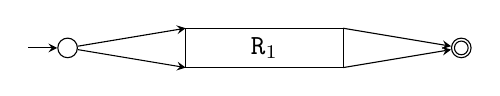
\begin{tikzpicture}
                    \node[circle, draw, inner sep=2.5pt] (q0) at (0, 0) {};
                    \draw (1.5, -0.25) rectangle (3.5, 0.25);
                    \node at (2.5, 0) {$\texttt{R}_1$};
                    \node[circle, draw, inner sep=2.5pt] (q1) at (5, 0) {};
                    \node[circle, draw, inner sep=1.75pt] at (5, 0) {};

                    \draw[-stealth] (-0.5, 0) -- (q0);
                    \draw[-stealth] (q0) -- (1.5, 0.25);
                    \draw[-stealth] (q0) -- (1.5, -0.25);
                    \draw[-stealth] (3.5, 0.25) -- (q1);
                    \draw[-stealth] (3.5, -0.25) -- (q1);
                \end{tikzpicture}
            \end{subfigure}
            \hfill
            \begin{subfigure}{0.4\textwidth}
                \centering
                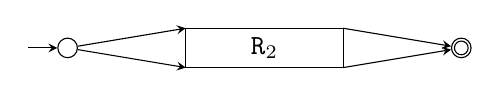
\begin{tikzpicture}
                    \node[circle, draw, inner sep=2.5pt] (q0) at (0, 0) {};
                    \draw (1.5, -0.25) rectangle (3.5, 0.25);
                    \node at (2.5, 0) {$\texttt{R}_2$};
                    \node[circle, draw, inner sep=2.5pt] (q1) at (5, 0) {};
                    \node[circle, draw, inner sep=1.75pt] at (5, 0) {};

                    \draw[-stealth] (-0.5, 0) -- (q0);
                    \draw[-stealth] (q0) -- (1.5, 0.25);
                    \draw[-stealth] (q0) -- (1.5, -0.25);
                    \draw[-stealth] (3.5, 0.25) -- (q1);
                    \draw[-stealth] (3.5, -0.25) -- (q1);
                \end{tikzpicture}
            \end{subfigure}
        \end{figure}
        Then, the NDFA for $\texttt{R}_1|\texttt{R}_2$ is the following:
        \begin{figure}[H]
            \centering
            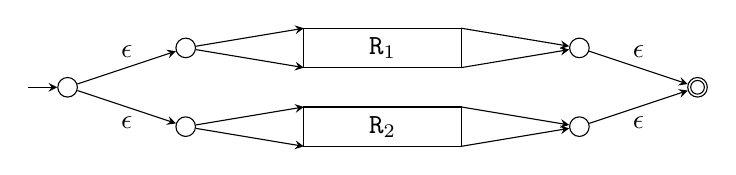
\begin{tikzpicture}
                \node[circle, draw, inner sep=2.5pt] (q0) at (0, 0) {};
                \draw (1.5, -0.25) rectangle (3.5, 0.25);
                \node at (2.5, 0) {$\texttt{R}_2$};
                \node[circle, draw, inner sep=2.5pt] (q1) at (5, 0) {};
                
                \node[circle, draw, inner sep=2.5pt] (q2) at (0, 1) {};
                \draw (1.5, 0.75) rectangle (3.5, 1.25);
                \node at (2.5, 1) {$\texttt{R}_1$};
                \node[circle, draw, inner sep=2.5pt] (q3) at (5, 1) {};

                \node[circle, draw, inner sep=2.5pt] (q4) at (-1.5, 0.5) {};
                \node[circle, draw, inner sep=2.5pt] (q5) at (6.5, 0.5) {};
                \node[circle, draw, inner sep=1.75pt] at (6.5, 0.5) {};

                \draw[-stealth] (-2, 0.5) -- (q4);
                \draw[-stealth] (q0) -- (1.5, 0.25);
                \draw[-stealth] (q0) -- (1.5, -0.25);
                \draw[-stealth] (3.5, 0.25) -- (q1);
                \draw[-stealth] (3.5, -0.25) -- (q1);
                
                \draw[-stealth] (q2) -- (1.5, 0.75);
                \draw[-stealth] (q2) -- (1.5, 1.25);
                \draw[-stealth] (3.5, 0.75) -- (q3);
                \draw[-stealth] (3.5, 1.25) -- (q3);

                \draw[-stealth] (q4) edge node[below] {$\epsilon$} (q0);
                \draw[-stealth] (q4) edge node[above] {$\epsilon$} (q2);
                \draw[-stealth] (q1) edge node[below] {$\epsilon$} (q5);
                \draw[-stealth] (q3) edge node[above] {$\epsilon$} (q5);
            \end{tikzpicture}
        \end{figure}

        \item The NDFA for \texttt{(R)} is the same as \texttt{R}.
        
        \item Let the NDFA for \texttt{R} be the following:
        \begin{figure}[H]
            \centering
            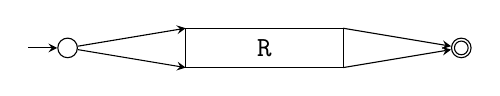
\begin{tikzpicture}
                \node[circle, draw, inner sep=2.5pt] (q0) at (0, 0) {};
                \draw (1.5, -0.25) rectangle (3.5, 0.25);
                \node at (2.5, 0) {\texttt{R}};
                \node[circle, draw, inner sep=2.5pt] (q1) at (5, 0) {};
                \node[circle, draw, inner sep=1.75pt] at (5, 0) {};

                \draw[-stealth] (-0.5, 0) -- (q0);
                \draw[-stealth] (q0) -- (1.5, 0.25);
                \draw[-stealth] (q0) -- (1.5, -0.25);
                \draw[-stealth] (3.5, 0.25) -- (q1);
                \draw[-stealth] (3.5, -0.25) -- (q1);
            \end{tikzpicture}
        \end{figure}
        Then, the NDFA for $\texttt{R}^*$ is the following:
        \begin{figure}[H]
            \centering
            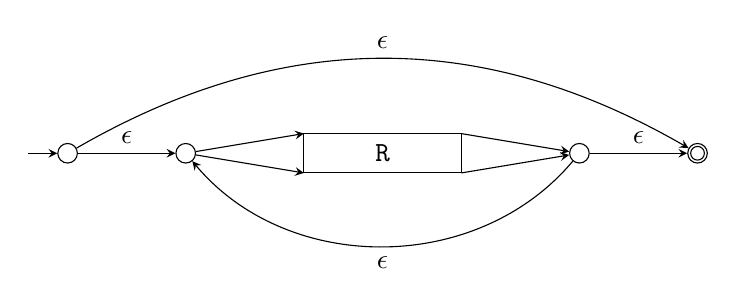
\begin{tikzpicture}
                \node[circle, draw, inner sep=2.5pt] (q0) at (0, 0) {};
                \draw (1.5, -0.25) rectangle (3.5, 0.25);
                \node at (2.5, 0) {\texttt{R}};
                \node[circle, draw, inner sep=2.5pt] (q1) at (5, 0) {};

                \node[circle, draw, inner sep=2.5pt] (q2) at (-1.5, 0) {};
                \node[circle, draw, inner sep=2.5pt] (q3) at (6.5, 0) {};
                \node[circle, draw, inner sep=1.75pt] at (6.5, 0) {};

                \draw[-stealth] (-2, 0) -- (q2);
                \draw[-stealth] (q0) -- (1.5, 0.25);
                \draw[-stealth] (q0) -- (1.5, -0.25);
                \draw[-stealth] (3.5, 0.25) -- (q1);
                \draw[-stealth] (3.5, -0.25) -- (q1);

                \draw[-stealth] (q2) edge node[above] {$\epsilon$} (q0);
                \draw[-stealth] (q1) edge node[above] {$\epsilon$} (q3);
                \draw[-stealth] (q1) edge[bend left=50] node[below] {$\epsilon$} (q0);
                \draw[-stealth] (q2) edge[bend left=30] node[above] {$\epsilon$} (q3);
            \end{tikzpicture}
        \end{figure}
    \end{itemize}

    We illustrate the construction of the NDFA for the regular expression $\texttt{(a}^*\texttt{b}|\texttt{ac)d}$. The NDFA for \texttt{a}, \texttt{b}, \texttt{ac} and \texttt{d} are the following:
    \begin{figure}[H]
        \centering
        \begin{subfigure}{0.3\textwidth}
            \centering
            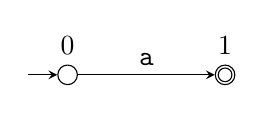
\begin{tikzpicture}
                \node[circle, draw, inner sep=2.5pt, label={90:0}] (q1) at (1.5, 0.5) {};
                \node[circle, draw, inner sep=2.5pt, label={90:1}] (q3) at (3.5, 0.5) {};
                \node[circle, draw, inner sep=1.75pt] at (3.5, 0.5) {};
    
                \draw[-stealth] (1, 0.5) -- (q1);
                \draw[-stealth] (q1) edge node[above] {\texttt{a}} (q3);
                \end{tikzpicture}
        \end{subfigure}
        \hfill
        \begin{subfigure}{0.3\textwidth}
            \centering
            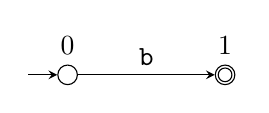
\begin{tikzpicture}
                \node[circle, draw, inner sep=2.5pt, label={90:0}] (q1) at (1.5, 0.5) {};
                \node[circle, draw, inner sep=2.5pt, label={90:1}] (q3) at (3.5, 0.5) {};
                \node[circle, draw, inner sep=1.75pt] at (3.5, 0.5) {};
    
                \draw[-stealth] (1, 0.5) -- (q1);
                \draw[-stealth] (q1) edge node[above] {\texttt{b}} (q3);
                \end{tikzpicture}
        \end{subfigure}
        \hfill
        \begin{subfigure}{0.3\textwidth}
            \centering
            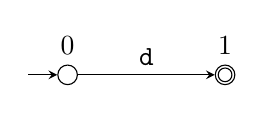
\begin{tikzpicture}
                \node[circle, draw, inner sep=2.5pt, label={90:0}] (q1) at (1.5, 0.5) {};
                \node[circle, draw, inner sep=2.5pt, label={90:1}] (q3) at (3.5, 0.5) {};
                \node[circle, draw, inner sep=1.75pt] at (3.5, 0.5) {};
    
                \draw[-stealth] (1, 0.5) -- (q1);
                \draw[-stealth] (q1) edge node[above] {\texttt{d}} (q3);
                \end{tikzpicture}
        \end{subfigure}
        \hfill
        \begin{subfigure}{0.5\textwidth}
            \centering
            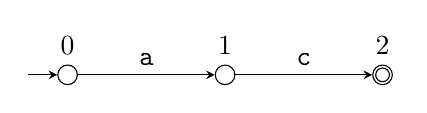
\begin{tikzpicture}
                \node[circle, draw, inner sep=2.5pt, label={90:0}] (q1) at (1.5, 0.5) {};
                \node[circle, draw, inner sep=2.5pt, label={90:1}] (q3) at (3.5, 0.5) {};
                \node[circle, draw, inner sep=2.5pt, label={90:2}] (q7) at (5.5, 0.5) {};
                \node[circle, draw, inner sep=1.75pt] at (5.5, 0.5) {};

                \draw[-stealth] (1, 0.5) -- (q1);
                \draw[-stealth] (q1) edge node[above] {\texttt{a}} (q3);
                \draw[-stealth] (q3) edge node[above] {\texttt{c}} (q7);
                \end{tikzpicture}
        \end{subfigure}
        \hfill
    \end{figure}
    \noindent So, the regular expression for $\texttt{a}^*$ is the following:
    \begin{figure}[H]
        \centering
        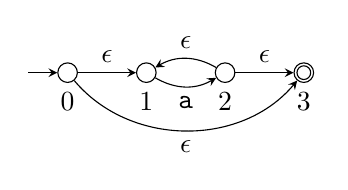
\begin{tikzpicture}
            \node[circle, draw, inner sep=2.5pt, label={-90:0}] (q2) at (1.5, -0.5) {};
            \node[circle, draw, inner sep=2.5pt, label={-90:1}] (q4) at (2.5, -0.5) {};
            \node[circle, draw, inner sep=2.5pt, label={-90:2}] (q5) at (3.5, -0.5) {};
            \node[circle, draw, inner sep=2.5pt, label={-90:3}] (q6) at (4.5, -0.5) {};
            \node[circle, draw, inner sep=1.75pt] at (4.5, -0.5) {};

            \draw[-stealth] (1, -0.5) -- (q2);
            \draw[-stealth] (q2) edge node[above] {$\epsilon$} (q4);
            \draw[-stealth] (q2) edge[bend right=50] node[below] {$\epsilon$} (q6);
            \draw[-stealth] (q4) edge[bend right] node[below] {\texttt{a}} (q5);
            \draw[-stealth] (q5) edge[bend right] node[above] {$\epsilon$} (q4);
            \draw[-stealth] (q5) edge node[above] {$\epsilon$} (q6);
        \end{tikzpicture}
    \end{figure}
    \noindent Now, the regular expression for $\texttt{a}^*\texttt{b}$ is the following:
    \begin{figure}[H]
        \centering
        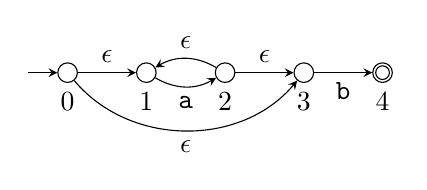
\begin{tikzpicture}
            \node[circle, draw, inner sep=2.5pt, label={-90:0}] (q2) at (1.5, -0.5) {};
            \node[circle, draw, inner sep=2.5pt, label={-90:1}] (q4) at (2.5, -0.5) {};
            \node[circle, draw, inner sep=2.5pt, label={-90:2}] (q5) at (3.5, -0.5) {};
            \node[circle, draw, inner sep=2.5pt, label={-90:3}] (q6) at (4.5, -0.5) {};
            \node[circle, draw, inner sep=2.5pt, label={-90:4}] (q8) at (5.5, -0.5) {};
            \node[circle, draw, inner sep=1.75pt] at (5.5, -0.5) {};

            \draw[-stealth] (1, -0.5) -- (q2);
            \draw[-stealth] (q2) edge node[above] {$\epsilon$} (q4);
            \draw[-stealth] (q2) edge[bend right=50] node[below] {$\epsilon$} (q6);
            \draw[-stealth] (q4) edge[bend right] node[below] {\texttt{a}} (q5);
            \draw[-stealth] (q5) edge[bend right] node[above] {$\epsilon$} (q4);
            \draw[-stealth] (q5) edge node[above] {$\epsilon$} (q6);
            \draw[-stealth] (q6) edge node[below] {\texttt{b}} (q8);
        \end{tikzpicture}
    \end{figure}
    \noindent Next, we construct the regular expression for $\texttt{a}^*\texttt{b|ac}$.
    \begin{figure}[H]
        \centering
        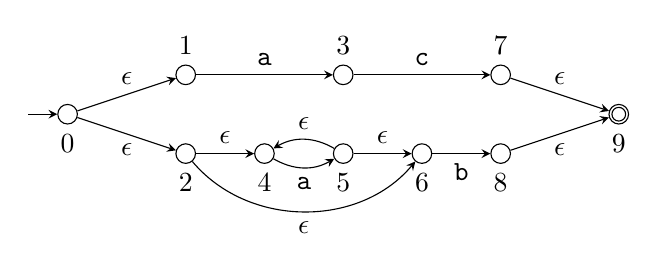
\begin{tikzpicture}
            \node[circle, draw, inner sep=2.5pt, label={-90:0}] (q0) at (0, 0) {};
            \node[circle, draw, inner sep=2.5pt, label={90:1}] (q1) at (1.5, 0.5) {};
            \node[circle, draw, inner sep=2.5pt, label={-90:2}] (q2) at (1.5, -0.5) {};
            \node[circle, draw, inner sep=2.5pt, label={90:3}] (q3) at (3.5, 0.5) {};
            \node[circle, draw, inner sep=2.5pt, label={-90:4}] (q4) at (2.5, -0.5) {};
            \node[circle, draw, inner sep=2.5pt, label={-90:5}] (q5) at (3.5, -0.5) {};
            \node[circle, draw, inner sep=2.5pt, label={-90:6}] (q6) at (4.5, -0.5) {};
            \node[circle, draw, inner sep=2.5pt, label={90:7}] (q7) at (5.5, 0.5) {};
            \node[circle, draw, inner sep=2.5pt, label={-90:8}] (q8) at (5.5, -0.5) {};
            \node[circle, draw, inner sep=2.5pt, label={-90:9}] (q9) at (7, 0) {};
            \node[circle, draw, inner sep=1.75pt] at (7, 0) {};

            \draw[-stealth] (-0.5, 0) -- (q0);
            \draw[-stealth] (q0) edge node[above] {$\epsilon$} (q1);
            \draw[-stealth] (q0) edge node[below] {$\epsilon$} (q2);
            \draw[-stealth] (q1) edge node[above] {\texttt{a}} (q3);
            \draw[-stealth] (q3) edge node[above] {\texttt{c}} (q7);
            \draw[-stealth] (q7) edge node[above] {$\epsilon$} (q9);
            \draw[-stealth] (q2) edge node[above] {$\epsilon$} (q4);
            \draw[-stealth] (q2) edge[bend right=50] node[below] {$\epsilon$} (q6);
            \draw[-stealth] (q4) edge[bend right] node[below] {\texttt{a}} (q5);
            \draw[-stealth] (q5) edge[bend right] node[above] {$\epsilon$} (q4);
            \draw[-stealth] (q5) edge node[above] {$\epsilon$} (q6);
            \draw[-stealth] (q6) edge node[below] {\texttt{b}} (q8);
            \draw[-stealth] (q8) edge node[below] {$\epsilon$} (q9);
        \end{tikzpicture}
    \end{figure}
    \noindent Finally, the regular expression for $\texttt{(a}^*\texttt{b|ac)d}$ is the following:
    \begin{figure}[H]
        \centering
        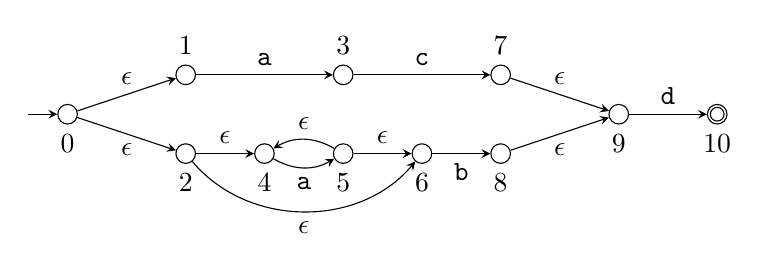
\begin{tikzpicture}
            \node[circle, draw, inner sep=2.5pt, label={-90:0}] (q0) at (0, 0) {};
            \node[circle, draw, inner sep=2.5pt, label={90:1}] (q1) at (1.5, 0.5) {};
            \node[circle, draw, inner sep=2.5pt, label={-90:2}] (q2) at (1.5, -0.5) {};
            \node[circle, draw, inner sep=2.5pt, label={90:3}] (q3) at (3.5, 0.5) {};
            \node[circle, draw, inner sep=2.5pt, label={-90:4}] (q4) at (2.5, -0.5) {};
            \node[circle, draw, inner sep=2.5pt, label={-90:5}] (q5) at (3.5, -0.5) {};
            \node[circle, draw, inner sep=2.5pt, label={-90:6}] (q6) at (4.5, -0.5) {};
            \node[circle, draw, inner sep=2.5pt, label={90:7}] (q7) at (5.5, 0.5) {};
            \node[circle, draw, inner sep=2.5pt, label={-90:8}] (q8) at (5.5, -0.5) {};
            \node[circle, draw, inner sep=2.5pt, label={-90:9}] (q9) at (7, 0) {};
            \node[circle, draw, inner sep=2.5pt, label={-90:10}] (q10) at (8.25, 0) {};
            \node[circle, draw, inner sep=1.75pt] at (8.25, 0) {};

            \draw[-stealth] (-0.5, 0) -- (q0);
            \draw[-stealth] (q0) edge node[above] {$\epsilon$} (q1);
            \draw[-stealth] (q0) edge node[below] {$\epsilon$} (q2);
            \draw[-stealth] (q1) edge node[above] {\texttt{a}} (q3);
            \draw[-stealth] (q3) edge node[above] {\texttt{c}} (q7);
            \draw[-stealth] (q7) edge node[above] {$\epsilon$} (q9);
            \draw[-stealth] (q9) edge node[above] {\texttt{d}} (q10);
            \draw[-stealth] (q2) edge node[above] {$\epsilon$} (q4);
            \draw[-stealth] (q2) edge[bend right=50] node[below] {$\epsilon$} (q6);
            \draw[-stealth] (q4) edge[bend right] node[below] {\texttt{a}} (q5);
            \draw[-stealth] (q5) edge[bend right] node[above] {$\epsilon$} (q4);
            \draw[-stealth] (q5) edge node[above] {$\epsilon$} (q6);
            \draw[-stealth] (q6) edge node[below] {\texttt{b}} (q8);
            \draw[-stealth] (q8) edge node[below] {$\epsilon$} (q9);
        \end{tikzpicture}
    \end{figure}

    By constructing the NDFA this way, we can guarantee that there is precisely one start and halt state. This follows from construction. Also, if the regular expression has length $r$, then there are at most $2r$ states in the NDFA. This is because every node has either one edge labelled by a character, or at most 2 edges labelled by $\epsilon$.

    We will now consider how the algorithm works. Given a string $s$ and a regular expression \texttt{R}, we first construct the NDFA for \texttt{R} as given by the algorithm above. Then, we run the algorithm by iterating through the characters in $s$. We keep track of all the states we can get to by following $s$ up to some index (and taking any $\epsilon$-edges). If we can reach the halting state at any point, we will have matched the string. We will make use of two functions to do so- \texttt{extendByEpsilon}, which extends the list of states by the ones that can be reached from this list and any $\epsilon$-edges; and \texttt{extendByChar}, which tells us what the next state would be if we took the character given from any of the states present.

    We illustrate the algorithm with an example- we have the regular expression $\texttt{(a}^*\texttt{b|ac)d}$ and the text \texttt{cabaabd}. The NDFA for the regular expression is the following:
    \begin{figure}[H]
        \centering
        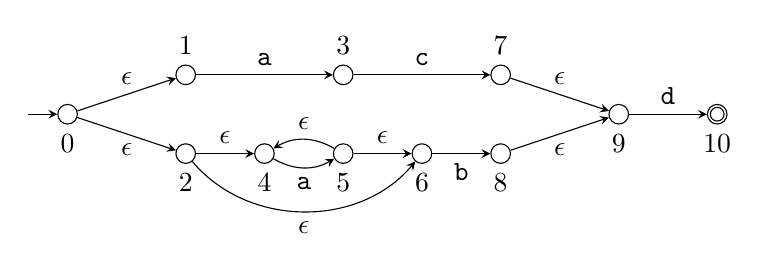
\begin{tikzpicture}
            \node[circle, draw, inner sep=2.5pt, label={-90:0}] (q0) at (0, 0) {};
            \node[circle, draw, inner sep=2.5pt, label={90:1}] (q1) at (1.5, 0.5) {};
            \node[circle, draw, inner sep=2.5pt, label={-90:2}] (q2) at (1.5, -0.5) {};
            \node[circle, draw, inner sep=2.5pt, label={90:3}] (q3) at (3.5, 0.5) {};
            \node[circle, draw, inner sep=2.5pt, label={-90:4}] (q4) at (2.5, -0.5) {};
            \node[circle, draw, inner sep=2.5pt, label={-90:5}] (q5) at (3.5, -0.5) {};
            \node[circle, draw, inner sep=2.5pt, label={-90:6}] (q6) at (4.5, -0.5) {};
            \node[circle, draw, inner sep=2.5pt, label={90:7}] (q7) at (5.5, 0.5) {};
            \node[circle, draw, inner sep=2.5pt, label={-90:8}] (q8) at (5.5, -0.5) {};
            \node[circle, draw, inner sep=2.5pt, label={-90:9}] (q9) at (7, 0) {};
            \node[circle, draw, inner sep=2.5pt, label={-90:10}] (q10) at (8.25, 0) {};
            \node[circle, draw, inner sep=1.75pt] at (8.25, 0) {};

            \draw[-stealth] (-0.5, 0) -- (q0);
            \draw[-stealth] (q0) edge node[above] {$\epsilon$} (q1);
            \draw[-stealth] (q0) edge node[below] {$\epsilon$} (q2);
            \draw[-stealth] (q1) edge node[above] {\texttt{a}} (q3);
            \draw[-stealth] (q3) edge node[above] {\texttt{c}} (q7);
            \draw[-stealth] (q7) edge node[above] {$\epsilon$} (q9);
            \draw[-stealth] (q9) edge node[above] {\texttt{d}} (q10);
            \draw[-stealth] (q2) edge node[above] {$\epsilon$} (q4);
            \draw[-stealth] (q2) edge[bend right=50] node[below] {$\epsilon$} (q6);
            \draw[-stealth] (q4) edge[bend right] node[below] {\texttt{a}} (q5);
            \draw[-stealth] (q5) edge[bend right] node[above] {$\epsilon$} (q4);
            \draw[-stealth] (q5) edge node[above] {$\epsilon$} (q6);
            \draw[-stealth] (q6) edge node[below] {\texttt{b}} (q8);
            \draw[-stealth] (q8) edge node[below] {$\epsilon$} (q9);
        \end{tikzpicture}
    \end{figure}
    \noindent At the start, we can only be at the starting state. Nonetheless, there are some $\epsilon$-edges that we can take from the start. This is shown below.
    \begin{figure}[H]
        \centering
        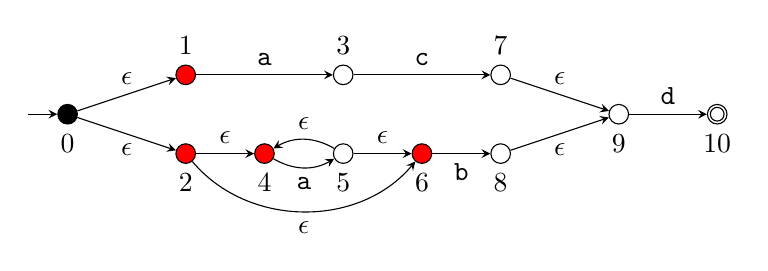
\begin{tikzpicture}
            \node[circle, draw, fill, inner sep=2.5pt, label={-90:0}] (q0) at (0, 0) {};
            \node[circle, draw, fill=red, inner sep=2.5pt, label={90:1}] (q1) at (1.5, 0.5) {};
            \node[circle, draw, fill=red, inner sep=2.5pt, label={-90:2}] (q2) at (1.5, -0.5) {};
            \node[circle, draw, inner sep=2.5pt, label={90:3}] (q3) at (3.5, 0.5) {};
            \node[circle, draw, fill=red, inner sep=2.5pt, label={-90:4}] (q4) at (2.5, -0.5) {};
            \node[circle, draw, inner sep=2.5pt, label={-90:5}] (q5) at (3.5, -0.5) {};
            \node[circle, draw, fill=red, inner sep=2.5pt, label={-90:6}] (q6) at (4.5, -0.5) {};
            \node[circle, draw, inner sep=2.5pt, label={90:7}] (q7) at (5.5, 0.5) {};
            \node[circle, draw, inner sep=2.5pt, label={-90:8}] (q8) at (5.5, -0.5) {};
            \node[circle, draw, inner sep=2.5pt, label={-90:9}] (q9) at (7, 0) {};
            \node[circle, draw, inner sep=2.5pt, label={-90:10}] (q10) at (8.25, 0) {};
            \node[circle, draw, inner sep=1.75pt] at (8.25, 0) {};

            \draw[-stealth] (-0.5, 0) -- (q0);
            \draw[-stealth] (q0) edge node[above] {$\epsilon$} (q1);
            \draw[-stealth] (q0) edge node[below] {$\epsilon$} (q2);
            \draw[-stealth] (q1) edge node[above] {\texttt{a}} (q3);
            \draw[-stealth] (q3) edge node[above] {\texttt{c}} (q7);
            \draw[-stealth] (q7) edge node[above] {$\epsilon$} (q9);
            \draw[-stealth] (q9) edge node[above] {\texttt{d}} (q10);
            \draw[-stealth] (q2) edge node[above] {$\epsilon$} (q4);
            \draw[-stealth] (q2) edge[bend right=50] node[below] {$\epsilon$} (q6);
            \draw[-stealth] (q4) edge[bend right] node[below] {\texttt{a}} (q5);
            \draw[-stealth] (q5) edge[bend right] node[above] {$\epsilon$} (q4);
            \draw[-stealth] (q5) edge node[above] {$\epsilon$} (q6);
            \draw[-stealth] (q6) edge node[below] {\texttt{b}} (q8);
            \draw[-stealth] (q8) edge node[below] {$\epsilon$} (q9);
        \end{tikzpicture}
    \end{figure}
    \noindent The reached states are given in black and the extended states are given in red. If the state 10 was already red (or black), the algorithm would be over. However, this is not the case, so we enter the main loop of the algorithm. We start by matching \texttt{c}. There is no \texttt{c} that can be reached from any of the black or the red states. At any point, we can restart and reach the initial state. Hence, the state of the NDFA remains as given above. Next, we move to \texttt{a}. In this case, we can match an \texttt{a} and get further in the NDFA:
    \begin{figure}[H]
        \centering
        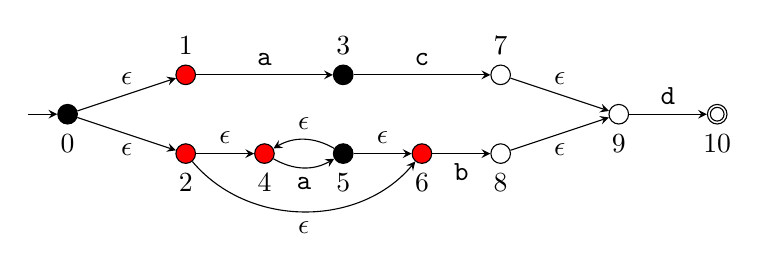
\begin{tikzpicture}
            \node[circle, draw, fill, inner sep=2.5pt, label={-90:0}] (q0) at (0, 0) {};
            \node[circle, draw, fill=red, inner sep=2.5pt, label={90:1}] (q1) at (1.5, 0.5) {};
            \node[circle, draw, fill=red, inner sep=2.5pt, label={-90:2}] (q2) at (1.5, -0.5) {};
            \node[circle, draw, fill, inner sep=2.5pt, label={90:3}] (q3) at (3.5, 0.5) {};
            \node[circle, draw, fill=red, inner sep=2.5pt, label={-90:4}] (q4) at (2.5, -0.5) {};
            \node[circle, draw, fill, inner sep=2.5pt, label={-90:5}] (q5) at (3.5, -0.5) {};
            \node[circle, draw, fill=red, inner sep=2.5pt, label={-90:6}] (q6) at (4.5, -0.5) {};
            \node[circle, draw, inner sep=2.5pt, label={90:7}] (q7) at (5.5, 0.5) {};
            \node[circle, draw, inner sep=2.5pt, label={-90:8}] (q8) at (5.5, -0.5) {};
            \node[circle, draw, inner sep=2.5pt, label={-90:9}] (q9) at (7, 0) {};
            \node[circle, draw, inner sep=2.5pt, label={-90:10}] (q10) at (8.25, 0) {};
            \node[circle, draw, inner sep=1.75pt] at (8.25, 0) {};

            \draw[-stealth] (-0.5, 0) -- (q0);
            \draw[-stealth] (q0) edge node[above] {$\epsilon$} (q1);
            \draw[-stealth] (q0) edge node[below] {$\epsilon$} (q2);
            \draw[-stealth] (q1) edge node[above] {\texttt{a}} (q3);
            \draw[-stealth] (q3) edge node[above] {\texttt{c}} (q7);
            \draw[-stealth] (q7) edge node[above] {$\epsilon$} (q9);
            \draw[-stealth] (q9) edge node[above] {\texttt{d}} (q10);
            \draw[-stealth] (q2) edge node[above] {$\epsilon$} (q4);
            \draw[-stealth] (q2) edge[bend right=50] node[below] {$\epsilon$} (q6);
            \draw[-stealth] (q4) edge[bend right] node[below] {\texttt{a}} (q5);
            \draw[-stealth] (q5) edge[bend right] node[above] {$\epsilon$} (q4);
            \draw[-stealth] (q5) edge node[above] {$\epsilon$} (q6);
            \draw[-stealth] (q6) edge node[below] {\texttt{b}} (q8);
            \draw[-stealth] (q8) edge node[below] {$\epsilon$} (q9);
        \end{tikzpicture}
    \end{figure}
    \noindent We still haven't reached the final state, so the algorithm has not yet terminated. We next match \texttt{b} and continue along.
    \begin{figure}[H]
        \centering
        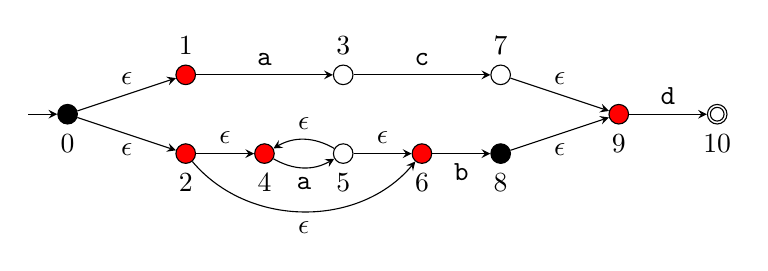
\begin{tikzpicture}
            \node[circle, draw, fill, inner sep=2.5pt, label={-90:0}] (q0) at (0, 0) {};
            \node[circle, draw, fill=red, inner sep=2.5pt, label={90:1}] (q1) at (1.5, 0.5) {};
            \node[circle, draw, fill=red, inner sep=2.5pt, label={-90:2}] (q2) at (1.5, -0.5) {};
            \node[circle, draw, inner sep=2.5pt, label={90:3}] (q3) at (3.5, 0.5) {};
            \node[circle, draw, fill=red, inner sep=2.5pt, label={-90:4}] (q4) at (2.5, -0.5) {};
            \node[circle, draw, inner sep=2.5pt, label={-90:5}] (q5) at (3.5, -0.5) {};
            \node[circle, draw, fill=red, inner sep=2.5pt, label={-90:6}] (q6) at (4.5, -0.5) {};
            \node[circle, draw, inner sep=2.5pt, label={90:7}] (q7) at (5.5, 0.5) {};
            \node[circle, draw, fill, inner sep=2.5pt, label={-90:8}] (q8) at (5.5, -0.5) {};
            \node[circle, draw, fill=red, inner sep=2.5pt, label={-90:9}] (q9) at (7, 0) {};
            \node[circle, draw, inner sep=2.5pt, label={-90:10}] (q10) at (8.25, 0) {};
            \node[circle, draw, inner sep=1.75pt] at (8.25, 0) {};

            \draw[-stealth] (-0.5, 0) -- (q0);
            \draw[-stealth] (q0) edge node[above] {$\epsilon$} (q1);
            \draw[-stealth] (q0) edge node[below] {$\epsilon$} (q2);
            \draw[-stealth] (q1) edge node[above] {\texttt{a}} (q3);
            \draw[-stealth] (q3) edge node[above] {\texttt{c}} (q7);
            \draw[-stealth] (q7) edge node[above] {$\epsilon$} (q9);
            \draw[-stealth] (q9) edge node[above] {\texttt{d}} (q10);
            \draw[-stealth] (q2) edge node[above] {$\epsilon$} (q4);
            \draw[-stealth] (q2) edge[bend right=50] node[below] {$\epsilon$} (q6);
            \draw[-stealth] (q4) edge[bend right] node[below] {\texttt{a}} (q5);
            \draw[-stealth] (q5) edge[bend right] node[above] {$\epsilon$} (q4);
            \draw[-stealth] (q5) edge node[above] {$\epsilon$} (q6);
            \draw[-stealth] (q6) edge node[below] {\texttt{b}} (q8);
            \draw[-stealth] (q8) edge node[below] {$\epsilon$} (q9);
        \end{tikzpicture}
    \end{figure}
    \noindent We have now reached state 9, but still not 10. So, we continue on with the algorithm. The next letter is \texttt{a}. We cannot go further from 8 or 9 using \texttt{a}, so we are back at the previous state:
    \begin{figure}[H]
        \centering
        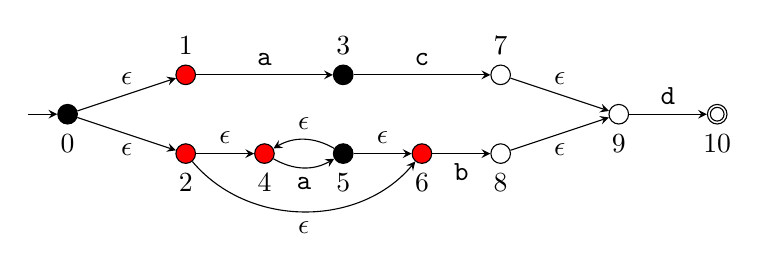
\begin{tikzpicture}
            \node[circle, draw, fill, inner sep=2.5pt, label={-90:0}] (q0) at (0, 0) {};
            \node[circle, draw, fill=red, inner sep=2.5pt, label={90:1}] (q1) at (1.5, 0.5) {};
            \node[circle, draw, fill=red, inner sep=2.5pt, label={-90:2}] (q2) at (1.5, -0.5) {};
            \node[circle, draw, fill, inner sep=2.5pt, label={90:3}] (q3) at (3.5, 0.5) {};
            \node[circle, draw, fill=red, inner sep=2.5pt, label={-90:4}] (q4) at (2.5, -0.5) {};
            \node[circle, draw, fill, inner sep=2.5pt, label={-90:5}] (q5) at (3.5, -0.5) {};
            \node[circle, draw, fill=red, inner sep=2.5pt, label={-90:6}] (q6) at (4.5, -0.5) {};
            \node[circle, draw, inner sep=2.5pt, label={90:7}] (q7) at (5.5, 0.5) {};
            \node[circle, draw, inner sep=2.5pt, label={-90:8}] (q8) at (5.5, -0.5) {};
            \node[circle, draw, inner sep=2.5pt, label={-90:9}] (q9) at (7, 0) {};
            \node[circle, draw, inner sep=2.5pt, label={-90:10}] (q10) at (8.25, 0) {};
            \node[circle, draw, inner sep=1.75pt] at (8.25, 0) {};

            \draw[-stealth] (-0.5, 0) -- (q0);
            \draw[-stealth] (q0) edge node[above] {$\epsilon$} (q1);
            \draw[-stealth] (q0) edge node[below] {$\epsilon$} (q2);
            \draw[-stealth] (q1) edge node[above] {\texttt{a}} (q3);
            \draw[-stealth] (q3) edge node[above] {\texttt{c}} (q7);
            \draw[-stealth] (q7) edge node[above] {$\epsilon$} (q9);
            \draw[-stealth] (q9) edge node[above] {\texttt{d}} (q10);
            \draw[-stealth] (q2) edge node[above] {$\epsilon$} (q4);
            \draw[-stealth] (q2) edge[bend right=50] node[below] {$\epsilon$} (q6);
            \draw[-stealth] (q4) edge[bend right] node[below] {\texttt{a}} (q5);
            \draw[-stealth] (q5) edge[bend right] node[above] {$\epsilon$} (q4);
            \draw[-stealth] (q5) edge node[above] {$\epsilon$} (q6);
            \draw[-stealth] (q6) edge node[below] {\texttt{b}} (q8);
            \draw[-stealth] (q8) edge node[below] {$\epsilon$} (q9);
        \end{tikzpicture}
    \end{figure}
    \noindent We are at the same state when we match the \texttt{a} again. 
    % TODO: Wrong!
    When we match \texttt{b}, we get the same state as above. Finally, we match \texttt{d}. In that case, the state of the NDFA is the following:
    \begin{figure}[H]
        \centering
        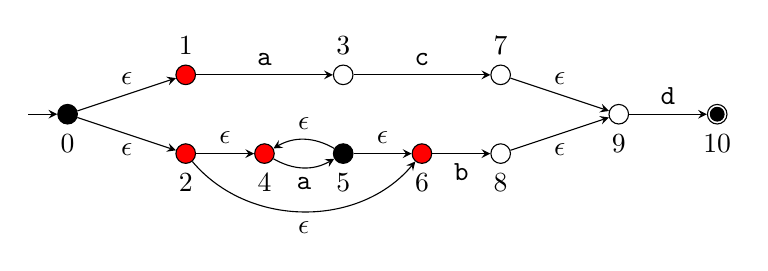
\begin{tikzpicture}
            \node[circle, draw, fill, inner sep=2.5pt, label={-90:0}] (q0) at (0, 0) {};
            \node[circle, draw, fill=red, inner sep=2.5pt, label={90:1}] (q1) at (1.5, 0.5) {};
            \node[circle, draw, fill=red, inner sep=2.5pt, label={-90:2}] (q2) at (1.5, -0.5) {};
            \node[circle, draw, inner sep=2.5pt, label={90:3}] (q3) at (3.5, 0.5) {};
            \node[circle, draw, fill=red, inner sep=2.5pt, label={-90:4}] (q4) at (2.5, -0.5) {};
            \node[circle, draw, fill, inner sep=2.5pt, label={-90:5}] (q5) at (3.5, -0.5) {};
            \node[circle, draw, fill=red, inner sep=2.5pt, label={-90:6}] (q6) at (4.5, -0.5) {};
            \node[circle, draw, inner sep=2.5pt, label={90:7}] (q7) at (5.5, 0.5) {};
            \node[circle, draw, inner sep=2.5pt, label={-90:8}] (q8) at (5.5, -0.5) {};
            \node[circle, draw, inner sep=2.5pt, label={-90:9}] (q9) at (7, 0) {};
            \node[circle, draw, inner sep=2.5pt, label={-90:10}] (q10) at (8.25, 0) {};
            \node[circle, draw, fill, inner sep=1.75pt] at (8.25, 0) {};

            \draw[-stealth] (-0.5, 0) -- (q0);
            \draw[-stealth] (q0) edge node[above] {$\epsilon$} (q1);
            \draw[-stealth] (q0) edge node[below] {$\epsilon$} (q2);
            \draw[-stealth] (q1) edge node[above] {\texttt{a}} (q3);
            \draw[-stealth] (q3) edge node[above] {\texttt{c}} (q7);
            \draw[-stealth] (q7) edge node[above] {$\epsilon$} (q9);
            \draw[-stealth] (q9) edge node[above] {\texttt{d}} (q10);
            \draw[-stealth] (q2) edge node[above] {$\epsilon$} (q4);
            \draw[-stealth] (q2) edge[bend right=50] node[below] {$\epsilon$} (q6);
            \draw[-stealth] (q4) edge[bend right] node[below] {\texttt{a}} (q5);
            \draw[-stealth] (q5) edge[bend right] node[above] {$\epsilon$} (q4);
            \draw[-stealth] (q5) edge node[above] {$\epsilon$} (q6);
            \draw[-stealth] (q6) edge node[below] {\texttt{b}} (q8);
            \draw[-stealth] (q8) edge node[below] {$\epsilon$} (q9);
        \end{tikzpicture}
    \end{figure}
    \noindent We have now reached the final state, meaning that we have found a match of the regular expression in the text ending at position. In this case, it is \texttt{abd}.

    The pseudocode for the algorithm is given below:
\begin{lstlisting}[language=pseudocode]
bool match(String string, NDFA ndfa) {
    Set<NDFAState> y = {ndfa.startState};
    Set<NDFAState> x = extendByEpsilon(y);
    
    // if the ndfa accepts the empty string, there os a match
    if (x.contains(ndfa.haltState)) {
        return true;
    }

    for (int i=0; i<string.length; i++) {
        y = extendByChar(x);
        y.add(ndfa.startState);

        x = extendByEpsilon(y);
        if (x.contains(ndfa.haltState)) {
            return true;
        }
    }

    return false;
}
\end{lstlisting}

    We will now consider the complexity of the algorithm. Let $r$ be the length of the regular expression and $t$ the length of the text. We loop at most $t$ times. Within each iteration, we use \texttt{extendByEpsilon} and \texttt{extendByChar}. The function \texttt{extendByChar} has complexity $O(n)$, where $n$ is the number of states in the NDFA- we compute \texttt{extendByChar} for each state in $O(1)$ time and combine the result. The function \texttt{extendByEpsilon} uses a depth first search approach, and has complexity $O(n+m)$, where $m$ is the number of edges. We know that an NDFA constructed as above has at most $2r$ states, and each state has at most 2 edges. Hence, the algorithm is $O(rt)$.
    \newpage

    \section{Longest Common Subsequence}
    In this section, we will consider computing the longest common subsequence in different ways. A subsequence of a string can be constructed by removing some characters from it, while maintaining the same order. We want to compute the longest common subsequence for two strings- its length and the actual subsequence. Typically, the longest common subsequence is not unique. Longest common substring is a measure of global similarity of two strings. 

    Our first approach for the computation is dynamic programming (DP). Here, we build the solution by computing smaller solutions. We will first look at iterative DP. When computing the LCS of two strings \texttt{s1} and \texttt{s2}, we have a table \texttt{t} with the  row label the characters in \texttt{s1} and the column label the characters in \texttt{s2}, including the empty character. We fill the first row and column with 0s, and recursively define
    \[\texttt{t}_{i, j} = \begin{cases}
        1 + \texttt{t}_{i-1, j-1} & \texttt{s1}[i-1] = \texttt{s2}[j-1] \\
        \max (\texttt{t}_{i-1, j}, \texttt{t}_{i, j-1}) & \text{otherwise}.
    \end{cases}\]
    The length of the LCS is given at the bottom right position. We illustrate this with an example- the table below is the DP table where we compute the LCS of \texttt{acbacadb} and \texttt{abadcda}:
    \begin{table}[H]
        \centering
        \begin{tabular}{c|ccccccccc}
            & $\epsilon$ & \texttt{a} & \texttt{c} & \texttt{b} & \texttt{a} & \texttt{c} & \texttt{a} & \texttt{d} & \texttt{b} \\
            \hline 
            $\epsilon$ & 0 & 0 & 0 & 0 & 0 & 0 & 0 & 0 & 0 \\
            \texttt{a} & 0 & 1 & 1 & 1 & 1 & 1 & 1 & 1 & 1 \\
            \texttt{b} & 0 & 1 & 1 & 2 & 2 & 2 & 2 & 2 & 2 \\
            \texttt{a} & 0 & 1 & 1 & 2 & 3 & 3 & 3 & 3 & 3 \\
            \texttt{d} & 0 & 1 & 1 & 2 & 3 & 3 & 3 & 4 & 4 \\
            \texttt{c} & 0 & 1 & 2 & 2 & 3 & 4 & 4 & 4 & 4 \\
            \texttt{d} & 0 & 1 & 2 & 2 & 3 & 4 & 4 & 5 & 5 \\
            \texttt{a} & 0 & 1 & 2 & 2 & 3 & 4 & 5 & 5 & 5 
        \end{tabular}
    \end{table}
    In the DP table, we have computed the LCS of different substrings of the 2 strings. For example, the LCS of any string with the empty string is 0- this is given in the first row and the first column. Moreover, the LCS of \texttt{acba} and \texttt{aba} is 3. In particular, the LCS of the two strings is 5- this is the bottom right entry.

    The algorithm for this version of LCS, to compute the length, is given below:
\begin{lstlisting}[language=pseudocode]
int lcs(String s1, String s2) {
    // initialise the 2D table with 0s
    List<List<int>> table = List(s1.length+1,List(s2.length+1,0));

    // use the formula to fill the table
    for (int i=1; i<s1.length+1; i++) {
        for (int j=1; j<s2.length+1; j++) {
            if (s1[i-1] == s2[j-1]) {
                table[i][j] = 1 + table[i-1][j-1];
            } else {
                table[i][j] = max(table[i-1][j], table[i][j-1]);
            }
        }
    }

    return table[s1.length][s2.length];
}
\end{lstlisting}
    We will now consider the complexity of the algorithm. It takes $O(1)$ time to fill in each entry of the table. So, the algorithm takes $O(mn)$ time and space, where $m$ and $n$ are the lengths of \texttt{s1} and \texttt{s2} respectively.

    We will now look at constructing the LCS using the DP table. We do this by backtracking from the bottom right entry- what choice did we make to get to that value. Every time we go up diagonally, we know that there was a match, so this character is part of the common subsequence. We illustrate this with the LCS for \texttt{acbacadb} and \texttt{abadcda}:
    \begin{table}[H]
        \centering
        \begin{tabular}{c|ccccccccc}
            & $\epsilon$ & \texttt{\color{blue} a} & \texttt{c} & \texttt{\color{blue} b} & \texttt{\color{blue} a} & \texttt{\color{blue} c} & \texttt{a} & \texttt{\color{blue} d} & \texttt{b} \\
            \hline 
            $\epsilon$ & {\color{red} 0} & 0 & 0 & 0 & 0 & 0 & 0 & 0 & 0 \\
            \texttt{\color{blue} a} & 0 & {\color{red} 1} & {\color{red} 1} & 1 & 1 & 1 & 1 & 1 & 1 \\
            \texttt{\color{blue} b} & 0 & 1 & 1 & {\color{red} 2} & 2 & 2 & 2 & 2 & 2 \\
            \texttt{\color{blue} a} & 0 & 1 & 1 & 2 & {\color{red} 3} & 3 & 3 & 3 & 3 \\
            \texttt{d} & 0 & 1 & 1 & 2 & {\color{red} 3} & 3 & 3 & 4 & 4 \\
            \texttt{\color{blue} c} & 0 & 1 & 2 & 2 & 3 & {\color{red} 4} & {\color{red} 4} & 4 & 4 \\
            \texttt{\color{blue} d} & 0 & 1 & 2 & 2 & 3 & 4 & 4 & {\color{red} 5} & {\color{red} 5} \\
            \texttt{a} & 0 & 1 & 2 & 2 & 3 & 4 & 5 & 5 & {\color{red} 5} 
        \end{tabular}
    \end{table}
    \noindent The values in red spell out how we got to the bottom right entry. The blue characters are the ones part of the common subsequence. In this case, it is \texttt{abacd}. This is not a unique traceback. For example, instead of going up from the bottom right position, we could have also gone to the left. This can lead to different common subsequences, but they will all have the maximum length possible.
    
    Instead of storing the entire table, we just need to store the previous row (and the diagonal value). This version of the algorithm is given below:
    % TODO: Add algorithm
    This algorithm still has $O(mn)$ time complexity, but the space complexity is $O(n)$. This approach does not allow us to construct the LCS. Nonetheless, there exists an algorithm that takes $O(mn)$ time complexity and $O(n)$ space and computes the actual LCS.
    
    When we construct the DP table iteratively, we compute all the entries. However, this might not be necessary. We can use a \emph{lazy} approach that computes all values that we need in order to find the bottom right entry on the table. This approach uses recursion. A naive approach to do so is the following:
\begin{lstlisting}[language=pseudocode]
// compute the lcs of s1[0..i] and s2[0..j]
int lcs(String s1, String s2, int i, int j) {
    if (i == 0 || j == 0) {
        return 0;
    } else if (s1[i-1] == s2[j-1]) {
        return 1 + lcs(s1, s2, i-1, j-1);
    } else {
        return max(lcs(s1, s2, i-1, j), lcs(s1, s2, i, j-1));
    }
}
\end{lstlisting}
    In this case, we do not necessarily compute all the entries in the DP table. However, this algorithm is very inefficient- it is exponential. This is because many computations are being repeated. For instance, the recursion trace of the values $(i, j)$ when we compute LCS for \texttt{caa} and \texttt{ab} is shown below:
    \begin{figure}[H]
        \centering
        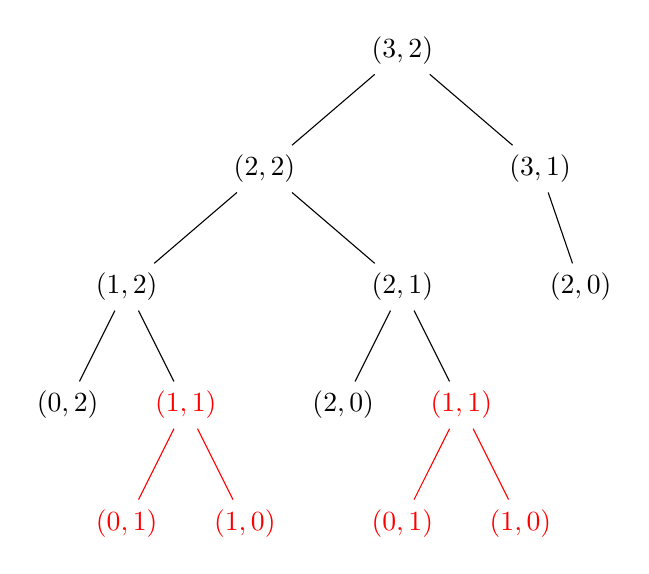
\begin{tikzpicture}[
            level 1/.style={sibling distance=3.5cm},
            level 3/.style={sibling distance=1.5cm},
        ]
            \node {$(3, 2)$}
            child {
                node {$(2, 2)$}
                child {
                    node {$(1, 2)$}
                    child {
                        node {$(0, 2)$}
                    }
                    child[red] {
                        node {$(1, 1)$}
                        child[red] {
                            node {$(0, 1)$}
                        }
                        child[red] {
                            node {$(1, 0)$}
                        }
                        edge from parent[black]
                    }
                }
                child {
                    node {$(2, 1)$}
                    child {
                        node {$(2, 0)$}
                    }
                    child[red] {
                        node {$(1, 1)$}
                        child[red] {
                            node {$(0, 1)$}
                        }
                        child[red] {
                            node {$(1, 0)$}
                        }
                        edge from parent[black]
                    }
                }
            }
            child {
                node {$(3, 1)$}
                child[right] {
                    node {$(2, 0)$}
                }
            };
        \end{tikzpicture}
    \end{figure}
    \noindent Even when we are comparing such simple strings, we have 3 common nodes in the recursion trace. Nonetheless, we can see that some combinations of $(i, j)$ are never computed, e.g. $(3, 0)$. 

    To improve the complexity of the recursive algorithm, we make use of \emph{memoisation}. Here, we use some space to keep track of which values we have already computed, i.e. we maintain an instance of the DP table. This version of the algorithm is given below:
\begin{lstlisting}[language=pseudocode]
// compute the lcs of s1[0..i] and s2[0..j] given the table of 
// values (initially -1)
int lcs(String s1, String s2, int i, int j, 
    List<List<int>> table) {
    // compute the value if needed
    if (table[i][j] == -1) {
        if (i == 0 || j == 0)  {
            table[i][j] = 0;
        } else if (s1[i-1] == s2[j-1]) {
            table[i][j] = 1 + lcs(s1, s2, i, j, table);
        } else {
            table[i][j] = max(
                lcs(s1, s2, i-1, j, table), 
                lcs(s1, s2, i, j-1, table)
            );
        }
    }

    return table[i][j];
}
\end{lstlisting}
    This algorithm has time and space complexity $O(mn)$ due to memoisation, and it only computes the necessary values. We can see this below, where we compute the LCS for \texttt{acbacadb} and \texttt{abadcda}:
    \begin{table}[H]
        \centering
        \begin{tabular}{c|ccccccccc}
            & $\epsilon$ & \texttt{\color{blue} a} & \texttt{c} & \texttt{\color{blue} b} & \texttt{\color{blue} a} & \texttt{\color{blue} c} & \texttt{a} & \texttt{\color{blue} d} & \texttt{b} \\
            \hline
            $\epsilon$ & 0 & -1 & 0 & 0 & -1 & 0 & -1 & 0 & -1 \\
            \texttt{\color{blue} a} & -1 & 1 & 1 & -1 & 1 & 1 & 1 & 1 & -1 \\
            \texttt{\color{blue} b} & 0 & 1 & 1 & 2 & 2 & 2 & 2 & 2 & 2 \\
            \texttt{\color{blue} a} & -1 & 1 & 1 & 2 & 3 & 3 & 3 & 3 & 3 \\
            \texttt{d} & 0 & 1 & 1 & 2 & 3 & 3 & 3 & 4 & 4 \\
            \texttt{\color{blue} c} & 0 & 1 & 2 & 2 & 3 & 4 & 4 & 4 & 4 \\
            \texttt{\color{blue} d} & 0 & 1 & 2 & 2 & 3 & 4 & -1 & 5 & 5 \\
            \texttt{a} & -1 & -1 & -1 & -1 & -1 & -1 & 5 & 5 & 5
        \end{tabular}
    \end{table}
    \noindent Clearly, not all the values have been computed, and we could still recover the LCS. However, we initialise the table with value \texttt{-1}- this means that we have already made use of the entire space. 
    
    To avoid this, we can declare the list and its size, and not initialise it with any values, and use pointers. In this case, we store the following values:
    \begin{itemize}
        \item the DP table, which is not initialised (and will have garbage values at the start);
        \item the pointers table, which is also not initialised, that has the same dimension as the DP table;
        \item a 1D list of pointers, with length equal to the product of the dimension of the DP table; and
        \item the number of values we have computed in the table.
    \end{itemize}
    The pointers table stores at which call the value at table was computed. The pointer list points back to the index in the DP table/pointer (we can convert the 2D index $(i, j)$ to the 1D index $i * m + j$, where $m$ is the length of \texttt{s1}). This way, we can avoid initialising the DP table. The algorithm now computes whether a value is correct as follows:
    \begin{itemize}
        \item we first check the pointers table at the given index. If it is less than 0 or bigger than the number of values we have computed, then it is not a valid value, i.e. we have not yet computed the value.
        \item otherwise, we check whether the 1D list of pointers. We know at this point that the value at this list of pointer is correct (it is one of the values that has been computed). So, if this pointer value points back to the same index in the table of pointers/values, we know that the value in the table is correct.
    \end{itemize}

    In this case, the algorithm is the following:
\begin{lstlisting}[language=pseudocode]
int lcs(String s1, String s2, int i, int j,
    List<List<int>> table, List<List<int>> tablePointers, 
    List<int> pointers1D) {
    bool isValid = false;
    int val = tablePointers[i][j];
    // to be valid, val must be between 0 and len = all inserted pointers in pointers1D
    if (val >= 0 && val < len) {
        // check whether the 1D pointer matches as well
        isValid = pointers1D[val] == i*s1.length+j;
    }

    if (!isValid) {
        if (i == 0 || j == 0)  {
            table[i][j] = 0;
        } else if (s1[i-1] == s2[j-1]) {
            table[i][j] = 1 + lcs(s1, s2, i, j, table);
            len++;
        } else {
            table[i][j] = max(
                lcs(s1, s2, i-1, j, table), 
                lcs(s1, s2, i, j-1, table)
            );
        }

        // change pointer values
        tablePointers[i][j] = len;
        pointers1D[len] = i*s1.length+j;
        len++;
    }

    return table[i][j];
}
\end{lstlisting}
    Although this algorithm takes more space, it avoids initialising the table of values- it is truly lazy. This technique is called \emph{virtual initialisation} (inserting values at unpredictable positions and deciding whether an entry is garbage).
    % TODO: Example?
    \newpage

    \section{Local Similarity in Strings}
    In the section above, we saw local common subsequence between two strings- this is a measure of how globally similar two strings are. We will now consider the concept of local string similarity, which will lead us to the Smith-Waterman algorithm.

    Consider the two strings \texttt{GAACTACATCATCTACTC} and \texttt{CGCATGTGACAGCTTCA}. A longest common subsequence of the two strings has length 10, given in the alignment below:
    \begin{table}[H]
        \centering
        \scalebox{0.85}{
            \begin{tabular}{cccccccccccccccccccccccccccccccccccccccc}
                & \texttt{G} &   & \texttt{A} & \texttt{A} & \texttt{C} & \texttt{T} & \texttt{A} & \texttt{C} & \texttt{A} & \texttt{T} & \texttt{C} & \texttt{A} & \texttt{T} & \texttt{C} & \texttt{T} & \texttt{A} &   & \texttt{C} & \texttt{T} &  & \texttt{C} \\
              \texttt{C} & \texttt{G} & \texttt{C} & \texttt{A} &   &   & \texttt{T} &   &   & \texttt{G} & \texttt{T} & \texttt{G} & \texttt{A} &   & \texttt{C} &   & \texttt{A} & \texttt{G} & \texttt{C} & \texttt{T} & \texttt{T} & \texttt{C} & \texttt{A}
            \end{tabular}
        }
    \end{table}
    \noindent The LCS is quite spread out. We can also ask whether there is a strongly similar contiguous block of characters that (almost) match within the two strings. For the two strings, the substrings \texttt{CATCTAC} and \texttt{CATGTGAC} are very similar. If we assign match a score of 1, and a mismatch (insertion, deletion or substitution) a score of $-1$, then these substrings would score 4; 2 differences and 6 matches.

    We can compute the local similarity using a DP approach. The recursive definition to compute the table \texttt{t} is given as follows:
    \[\texttt{t}_{i, j} = \begin{cases}
        1 + \texttt{t}_{i-1, j-1} & s1[i-1] = s2[j-1] \\
        \max(0, \max(\texttt{t}_{i-1, j-1}, \texttt{t}_{i, j-1}, \texttt{t}_{i-1, j}) - 1) & \text{otherwise}.
    \end{cases}\]
    In the base case, we have $\texttt{t}_{i, 0} = 0$ and $\texttt{t}_{0, j} = 0$. Since the empty string is always locally similar between the two strings, and has length 0, the local similarity is always non-negative. If there is a match, the score increases by 1. Otherwise, the score decreases by 1 from the best one corresponding to a mismatch, but stays bigger than 0. We keep track of the best score in the table- this corresponds to the end of the locally similar substrings.


    We will illustrate the DP table with an example. Below, we compute the local similarity for \texttt{ADGGAGTAC} and \texttt{DGACTA}:
    \begin{table}[H]
        \centering
        \begin{tabular}{c|ccccccccccc}
            & $\epsilon$ & \texttt{A} & \texttt{D} & \texttt{G} & \texttt{G} & \texttt{A} & \texttt{G} & \texttt{T} & \texttt{A} & \texttt{C} \\
            \hline
            $\epsilon$ & 0 & 0 & 0 & 0 & 0 & 0 & 0 & 0 & 0 & 0 \\
            \texttt{D} & 0 & 0 & 1 & 0 & 0 & 0 & 0 & 0 & 0 & 0 \\
            \texttt{G} & 0 & 0 & 0 & 2 & 1 & 0 & 1 & 0 & 0 & 0 \\
            \texttt{A}& 0 & 1 & 0 & 1 & 1 & 2 & 1 & 0 & 1 & 0 \\
            \texttt{C} & 0 & 0 & 0 & 0 & 0 & 1 & 1 & 0 & 0 & 2 \\
            \texttt{T} & 0 & 0 & 0 & 0 & 0 & 0 & 0 & 2 & 1 & 1 \\
            \texttt{A} & 0 & 1 & 0 & 0 & 0 & 1 & 0 & 1 & {\color{red} 3} & 2
        \end{tabular}
    \end{table}
    \noindent In this case, the best score is 3. In this case, there is a unique occurrence of the value 3; in general, this need not be the case. If one pair of strongly similar substrings is a substring of another pair, we say that the shorter one is a \emph{contraction} of the longer one, and that the longer one is not \emph{minimal}.
    
    We can trace back from this value to the score 0 to find the strongly similar substrings.
    \begin{table}[H]
        \centering
        \begin{tabular}{c|ccccccccccc}
            & $\epsilon$ & \texttt{A} & \texttt{D} & \texttt{G} & \texttt{G} & \texttt{A} & \texttt{G} & \texttt{T} & \texttt{A} & \texttt{C} \\
            \hline
            $\epsilon$ & 0 & 0 & 0 & 0 & 0 & 0 & 0 & 0 & 0 & 0 \\
            \texttt{D} & 0 & 0 & 1 & {\color{red} 0} & 0 & 0 & 0 & 0 & 0 & 0 \\
            \texttt{G} & 0 & 0 & 0 & 2 & {\color{red} 1} & 0 & 1 & 0 & 0 & 0 \\
            \texttt{A}& 0 & 1 & 0 & 1 & 1 & {\color{red} 2} & 1 & 0 & 1 & 0 \\
            \texttt{C} & 0 & 0 & 0 & 0 & 0 & 1 & {\color{red} 1} & 0 & 0 & 2 \\
            \texttt{T} & 0 & 0 & 0 & 0 & 0 & 0 & 0 & {\color{red} 2} & 1 & 1 \\
            \texttt{A} & 0 & 1 & 0 & 0 & 0 & 1 & 0 & 1 & {\color{red} 3} & 2
        \end{tabular}
    \end{table}
    \noindent Using this traceback, we can compute the alignment of the two locally similar substrings:
    \begin{table}[H]
        \centering
        \begin{tabular}{cccccccc}
            \texttt{G} & \texttt{A} & \texttt{\color{red} G} & \texttt{T} & \texttt{A} \\
            \texttt{G} & \texttt{A} & \texttt{\color{red} C} & \texttt{T} & \texttt{A}
        \end{tabular}
    \end{table}
    \noindent It has score 3 since there are 4 matching characters and 1 mismatch. The indices of the locally similar substrings are called the \emph{extents}. In this case, the extent in \texttt{s1} is 1-7, and the extent in \texttt{s2} is 1-6.
    
    The following is the iterative DP algorithm for the Smith-Waterman algorithm, computing the highest score.
\begin{lstlisting}[language=pseudocode]
int smithWaterman(String s1, String s2) {
    int bestScore = 0;
    List<List<int>> values = List(s1.length+1, 
        List(s2.length+1, 0));

    for (int i=1; i<s1.length+1; i++) {
        for (int j=1; j<s2.length+1; j++) {
            if (s1[i-1] == s2[j-1]) {
                values[i][j] = 1 + values[i-1][j-1];

                if (values[i][j] > bestScore) {
                    bestScore = values[i][j];
                }
            } else {
                values[i][j] = max(
                    values[i-1][j-1], values[i][j-1],
                    values[i-1][j], 0
                );
            }
        }
    }

    return bestScore;
}
\end{lstlisting}
    We can extend the algorithm to also do the traceback. This allows us to compute the extent (and the alignment) of the local similarity.

    We now consider the complexity of the algorithm. The time complexity of the algorithm in any DP version is $O(mn)$. The space complexity can be lowered to $O(n)$ by only storing the current/previous row (in the same array), along with the diagonal value. We can extend the algorithm to also compute all the positions where the best score occurs- this can increase the space complexity in the $O(n)$ algorithm to $O(n+r)$, where $r$ is the maximum length of the best scoring points at any point during the algorithm.

    We can also get the $O(n+r)$ complexity when we compute the extent in the two strings. The 2D index of the best score represents the end of the extent; we need to traceback in order to find the start of the extent (called the \emph{origin}) in the two strings. We do this using a (space-optimised) DP algorithm, keeping the table \texttt{x} for the origin in \texttt{s1}, and \texttt{y} for the origin in \texttt{s2}. The position, in the two cases is computed by the following recurrence relations:
\[\texttt{x}_{i, j} = \begin{cases}
    i & \texttt{t}_{i, j} = 0 \\
    \texttt{x}_{i-1, j-1} & s1[i-1] = s2[j-1] \\
    \texttt{x}_{i-1, j} & \texttt{t}_{i, j} = 1 + \texttt{t}_{i-1, j} \\
    \texttt{x}_{i, j-1} & \texttt{t}_{i, j} = 1 + \texttt{t}_{i, j-1} \\
    \texttt{x}_{i-1, j-1} & \texttt{t}_{i, j} = 1 + \texttt{t}_{i-1, j-1}, 
    \end{cases}
    \texttt{y}_{i, j} =  \begin{cases}
    j & \texttt{t}_{i, j} = 0 \\
    \texttt{y}_{i-1, j-1} & s1[i-1] = s2[j-1] \\
    \texttt{y}_{i-1, j} & \texttt{t}_{i, j} = 1 + \texttt{t}_{i-1, j} \\
    \texttt{y}_{i, j-1} & \texttt{t}_{i, j} = 1 + \texttt{t}_{i, j-1} \\
    \texttt{y}_{i-1, j-1} & \texttt{t}_{i, j} = 1 + \texttt{t}_{i-1, j-1}.
\end{cases}\]
    \noindent This equation follows from how we compute the origin of the best score:
    \begin{itemize}
        \item if the value is 0, then we are at the origin, i.e. if $\texttt{t}_{i, j} = 0$, then $\texttt{x}_{i, j} = i$;
        \item if the values match, then we incremented the diagonal score, meaning that the origin is the same as for the diagonal, i.e. if $s1[i-1] = s2[j-1]$, then $\texttt{x}_{i, j} = \texttt{x}_{i-1, j-1}$;
        \item if we decreased the value in case of a mismatch, then we take the score that we took. In this case, we give precedence to deletion, then insertion and finally substitution; this order can be changed to get the right extent.
    \end{itemize}

    We saw above that the following was the DP table used to find best scoring local similarity for \texttt{ADGGAGTAC} and \texttt{DGACTA}:
    \begin{table}[H]
        \centering
        \begin{tabular}{c|ccccccccccc}
            & $\epsilon$ & \texttt{A} & \texttt{D} & \texttt{G} & \texttt{G} & \texttt{A} & \texttt{G} & \texttt{T} & \texttt{A} & \texttt{C} \\
            \hline
            $\epsilon$ & 0 & 0 & 0 & 0 & 0 & 0 & 0 & 0 & 0 & 0 \\
            \texttt{D} & 0 & 0 & 1 & 0 & 0 & 0 & 0 & 0 & 0 & 0 \\
            \texttt{G} & 0 & 0 & 0 & 2 & 1 & 0 & 1 & 0 & 0 & 0 \\
            \texttt{A}& 0 & 1 & 0 & 1 & 1 & 2 & 1 & 0 & 1 & 0 \\
            \texttt{C} & 0 & 0 & 0 & 0 & 0 & 1 & 1 & 0 & 0 & 2 \\
            \texttt{T} & 0 & 0 & 0 & 0 & 0 & 0 & 0 & 2 & 1 & 1 \\
            \texttt{A} & 0 & 1 & 0 & 0 & 0 & 1 & 0 & 1 & {\color{red} 3} & 2
        \end{tabular}
    \end{table}
    \noindent The position of the best score is $(7, 5)$. We will now find the $(x, y)$ origin values for this computation:
    \begin{table}[H]
        \centering
        \scalebox{0.9}{
        \begin{tabular}{c|ccccccccccc}
            & $\epsilon$ & \texttt{A} & \texttt{D} & \texttt{G} & \texttt{G} & \texttt{A} & \texttt{G} & \texttt{T} & \texttt{A} & \texttt{C} \\
            \hline
            $\epsilon$ & (0, 0) & (1, 0) & (2, 0) & (3, 0) & (4, 0) & (5, 0) & (6, 0) & (7, 0) & (8, 0) & (9, 0) \\
            \texttt{D} & (0, 1) & (1, 1) & (1, 0) & (3, 1) & (4, 1) & (5, 1) & (6, 1) & (7, 1) & (8, 1) & (9, 1) \\
            \texttt{G} & (0, 2) & (1, 2) & (2, 2) & (1, 0) & (3, 1) & (5, 2) & (5, 1) & (7, 2) & (8, 2) & (9, 2) \\
            \texttt{A} & (0, 3) & (0, 2) & (2, 3) & (1, 0) & (1, 0) & (3, 1) & (3, 1) & (7, 3) & (7, 2) & (9, 3) \\
            \texttt{C} & (0, 4) & (1, 4) & (2, 4) & (3, 4) & (4, 4) & (3, 1) & (3, 1) & (7, 4) & (8, 4) & (7, 2) \\
            \texttt{T} & (0, 5) & (1, 5) & (2, 5) & (3, 5) & (4, 5) & (5, 5) & (6, 5) & (3, 1) & (3, 1) & (7, 2) \\
            \texttt{A} & (0, 6) & (0, 5) & (2, 6) & (3, 6) & (4, 6) & (4, 5) & (6, 6) & (3, 1) & {\color{red} (3, 1)} & (3, 1)
        \end{tabular}}
    \end{table}
    \noindent So, we find that the extents are $s1[3..7]$ and $s2[1..5]$.

\end{document}